% -*- program: xelatex -*- %
\documentclass[language=english,noinputenc]{wiwwuwordrprt}

\usepackage{wiwwubildertabellen}
\usepackage{wiwwumathe}
\usepackage{wiwwulistings}
\usepackage{wiwwuabkuerzungen}
\usepackage{etoolbox}
\usepackage{blindtext}
\usepackage{minted}
\usepackage{booktabs}
\usepackage{enumitem}
\usepackage{pdfpages}

\usepackage{tikz-uml}
\usepackage{forest}
\usetikzlibrary{trees, arrows,shadows, positioning,chains,fit,shapes,calc, math, automata}
\usepackage{pgf-umlsd}


\usepackage{adjustbox}

\newcolumntype{R}[2]{%
    >{\adjustbox{angle=#1,lap=\width-(#2)}\bgroup}%
    l%
    <{\egroup}%
}
\newcommand*\rot{\multicolumn{1}{R{80}{1em}}}

\forestset{
  dir tree/.style={
    for tree={
      parent anchor=south west,
      child anchor=west,
      anchor=mid west,
      inner ysep=1pt,
      grow'=0,
      align=left,
      edge path={
        \noexpand\path [draw, \forestoption{edge}] (!u.parent anchor) ++(0.75em,0) |- (.child anchor)\forestoption{edge label};
      },
      font=\sffamily,
      if n children=0{}{
        delay={
          prepend={[,phantom, calign with current]}
        }
      },
      fit=band,
      before computing xy={
        l=1.5em
      }
    },
  }
}


\usepackage{amssymb}
\usepackage{pifont}
\newcommand{\cmark}{\ding{51}}%
\newcommand{\xmark}{\ding{55}}%
\newcommand{\ja}{\tiny{\cmark}}

\newlist{tabitemize}{itemize}{1}
\setlist[tabitemize]{label=\textbullet,nosep,after=\strut,leftmargin=*}

\newcolumntype{C}[1]{>{\centering\arraybackslash}m{#1}}
\newcolumntype{T}[1]{>{\riggedright\arraybackslash}p{#1}}

\usemintedstyle{tango}
\robustify\textellipsis
% \addtokomafont{section}{\clearpage}

\usepackage{fontspec}
\setmainfont[
  Ligatures=TeX,
  BoldFont={Crimson Text Bold},
  ItalicFont={Crimson Text Italic},
  BoldItalicFont={Crimson Text Bold Italic}
  ]{Crimson Text}
\setmonofont[Scale=0.9]{Source Code Pro}
\setsansfont{Lato}

\newcommand{\tabitem}{~~\llap{--}~~}

  \setThema{Prototypical Development of a\\Docker-based Workflow Management System}
  \setTyp{Masterthesis}
  \setFachgebiet{}
  \setLehrstuhl{Department of Information Systems --- Chair for Practical Computer Science}
  \setThemensteller{Prof.\ Dr.\ Herbert Kuchen}
  \setBetreuer{MScIS Vincent von Hof}
  \setAutor{Lars Greiving}
  \setStrasse{Dettenstraße 4}
  \setOrt{48147 Münster}
  \setTelefonnummer{+49-176 704 253 17}
  \setEMail{\textit{l\_grei02@uni-muenster.de}} % optional
  % leider vervollständigen einige PDF-Reader die E-Mail-Adresse mit einem Link. Wäre halb so wild, wenn sie dabei nicht den Teil *VOR* einem Punkt (also max bei max.mustermann@uni-muenster.de) übersehen würden. Dann lieber manuell den Link eintragen: \href{mailto:max.mustermann@uni-muenster.de}{max.mustermann@uni-muenster.de}
  \setAbgabetermin{2016-02-24}

\begin{document}
  \newlength{\customtabwidth}
  \setlength{\customtabwidth}{\textwidth}
  \addtolength{\customtabwidth}{-\tabcolsep}
  \captionsetup{justification=centering}

  \EinfTitelseite

  %Verzeichnisse
  \pagenumbering{Roman} % Seitennummerierung durch roemische Ziffern
  \tableofcontents
  \listoffigures
  \listoftables

  % -*- root: ../../main.tex -*- %

\begin{AbkVerzeichnis}
  \acro{AMQP}{Advanced Message Queuing Protocol}
  \acro{API}{Application Programming Interface}
  \acro{cgroups}{control groups}
  \acro{CLI}{command line interface}
  \acro{CoW}{Copy-on-Write}
  \acro{CRUD}{Create, Read, Update, Delete}
  \acro{ESB}{Enterprise Service Bus}
  \acro{GUI}{Graphical User Interface}
  \acro{HTML}{HyperText Markup Language}
  \acro{HTTP}{Hypertext Transfer Protocol}
  \acro{ID}{Identifier}
  \acro{IP}{Internet Protocol}
  \acro{IT}{Information Techonology}
  \acro{JSON}{JavaScript Object Notation}
  \acro{LXC}{Linux Containers}
  \acro{MOM}{Message-oriented Middleware}
  \acro{MSA}{Micro-services Architecture}
  \acro{NFS}{Network File System}
  \acro{OASIS}{Organization for the Advancement of Structured Information Standards}
  \acro{OS}{Operating System}
  \acro{P2P}{peer-to-peer}
  \acro{PaaS}{Platform as a Service}
  \acro{PID}{Process \ac{ID}}
  \acro{REST}{Representational State Transfer}
  \acro{RoR}{Ruby on Rails}
  \acro{SaaS}{Software as a Service}
  \acro{SOA}{Service-oriented Architecture}
  \acro{UI}{User Interface}
  \acro{WfMC}{Workflow Management Coalition}
  \acro{WfMS}{Workflow Management System}
  \acro{WFM}{Workflow Management}
  \acro{WSDL}{Web Services Description Language}
  \acro{YAML}{YAML Ain’t Markup Language}
\end{AbkVerzeichnis}

  %% -*- root: ../../main.tex -*- %

\begin{Verzeichnis}{Symbolverzeichnis}
  \VerzEintrag{$a_0$}{Anschaffungsauszahlung in $t = 0$}
  \VerzEintrag{$C$}{Kapitalwert}
  \VerzEintrag{$dt$}{Einzahlungsüberschuss in bezug auf $t$}
  \VerzEintrag{$i$}{Kalkulationszinsfuß}
  \VerzEintrag{$n$}{Nutzungsdauer}
  \VerzEintrag{$q$}{Zinsfaktor $1 + i$}
  \VerzEintrag{$r_s$}{Abstand der Stufe s in cm vom Seitenrand}
  \VerzEintrag{$s$}{Stufenindex}
  \VerzEintrag{$t$}{Periodenindex}
\end{Verzeichnis}


  \clearpage
  % -*- root: ../../main.tex -*- %

\begin{abstract}
\end{abstract}


  \pagenumbering{arabic} % Seitennummerierung durch arabische Ziffern

  \chapter{Introduction and Motivation} % (fold)
    \label{cha:introduction_and_motivation}
    % -*- root: ../../main.tex -*- %

Organizations perform temporal and logical sequences of actions that help to interact with business relevant entities -- business processes -- with the objective to reach their business goals. If these processes are coordinated in an automated way, they are also called \emph{workflows}. \acp{WfMS} are designed to support the definition, execution and monitoring of these workflows.

In the past years, enterprises reacted to their need for increased computational power by making use of \ac{IT} infrastructure and software applications that are offered as services. These offers are known as \ac{PaaS} and \ac{SaaS} \cite[p.~606]{Buyya2009Cloud}. To be able run software in an environment enhanced with such services, various approaches have been presented. One of them is the use of software containers.
Software containers provide a way of packaging and executing processes that isolates the application from the underlying \ac{OS} of a computer and other processes that run on it.
%They enable developers to supply their applications with specifically tailored runtime environments without having to worry about conflicting versions of dependencies. \cite{}
The concept of software containers is no new notion: an early predecessor was the \texttt{chroot} command, which dates back to 1979, \emph{software jails} followed in 1998 \cite{Bernstein2014Containers}.
In the second decade of the \nth{21} century, solutions like Rocket, LXD, and Docker emerged, which aim at the introduction of standardized, re-usable software containers, usually in combination with tools for their management. Among these solutions, Docker is very popular. In the beginning of 2016, it was the \nth{20} most ``starred'' repository on the source code management platform \emph{GitHub} -- ranking four positions behind the Linux kernel repository \cite{Github2016Repositories}. Docker comes with a set of utilities, which extend its main container-related functionality.

With regards to the challenges that heterogenous and distributed \ac{IT} environments as described above impose on \acp{WfMS} -- \eg the distribution of workflows to their location of enactment, the requirement to be able to adapt to increasing workload, or manage the remote execution of tasks -- it could be of interest to fathom possible benefits that may arise from the use of the Docker tool set in the context of these \acp{WfMS}. The primary objectives of the thesis at hand are thus to address the following questions and to derive artifacts from the findings that may serve as a foundation for the conceptualization and implementation of upcoming \acp{WfMS}:

\begin{description}
  \item[RQ1:] How can Docker leverage the deployment and execution of workflows in a distributed environment?
  \item[RQ2:] Which decisions in software architecture and software design of a WFMS are complemented by Docker's functionality?
\end{description}

The structure of this thesis follows the design science research process suggested by Peffers et al. \cite[pp.~89-92]{Peffers2007Design}. The research problem is identified in this very chapter and the chapters \ref{cha:workflow_management_systems} and \ref{cha:docker}, in which the fundamental concepts of Docker and \acp{WfMS} are introduced.
Based on considerations drawn from these concepts, the objectives of a solution are inferred and a prototype is designed in Chapter~\ref{cha:solution_design}. The implementation and usage of the prototype are described in Chapter~\ref{cha:implementation}. In Chapter~\ref{cha:evaluation}, the developed mechanism and the prototype are evaluated. Finally, the findings of this thesis are summarized and suggestions for subsequent research are presented in Chapter\ref{cha:conclusion}.

** related work

    % chapter introduction_and_motivation (end)

  \chapter{Workflow Management Systems} % (fold)
    \label{cha:workflow_management_systems}
    In this chapter, the concepts of workflows and workflow management systems will be briefly introduced and related to each other.
    There is a plethora of term definitions and deviating understandings of workflows and the concepts related to them \cite{Casati1999Specification}.
    In large parts, the concepts presented here thus rely on specifications published by the \ac{WFMC}, a consortium of workflow management software vendors, researchers in the field of workflow management and \ac{WfMS} users, as they represent some form of consensus.

    The identified use cases and properties will be used in \ref{sec:determination_of_objectives} to identify objectives for the architecture. Also, they will be the reference to which the final architecture developed in this thesis is compared against.
    % -*- root: ../../main.tex -*- %

\section{Concepts} % (fold)
\label{sec:concepts}

  \subsection{Workflow} % (fold)
  \label{sub:workflow}
    In order to achieve their business goals, organizations perform temporal and logical sequences of tasks that help to interact with business relevant entities. These sequences are known as \emph{business processes}. If the logic that controls the processes is performed in an automated way, \eg by an information system, one refers to the processes as \emph{workflows} \cite{Becker1999Identifying,Hollingsworth1995Wfmc}. The \ac{WfMC} defines workflows as ``the computerized facilitation or automation of a business process, in whole or part'' \cite{Hollingsworth1995Wfmc}.

    \emph{Process activities} are the atomic steps that processes consist of. The \ac{WfMC} differentiates between \emph{manual activities} and \emph{workflow activities}. The former are activities that involve user interaction in order to be completed, while the latter are automated and require no interaction \cite{Hollingsworth1995Wfmc}. As the term ``workflow activity'' might be misunderstood as ``any activity belonging to a workflow'', in the following the term \emph{automated activity} will be used instead.

    % go into backgrounds of activities, concept: atomic piece of work -> later: analogy to docker container
  % subsection workflow (end)

  \subsection{Process definition} % (fold)
  \label{sub:process_definition}
    In order to be able to execute workflows, the underlying business processes must be machine processable and thus have to be formalized to an abstracted model \cite{Hollingsworth1995Wfmc}. This model is usually called \emph{process definition} and stored in form of some high-level programming language construct \cite{Hollingsworth1995Wfmc,Wutke2008Model}.
    The process definitions typically consist of a collection of activities with additional metadata such as associated applications or participants, and a set of rules which determine the execution order of these activities \cite{Hollingsworth1995Wfmc}. They further may contain references to other processes, which are treated as a single activity in the process definition \cite{Hollingsworth1995Wfmc,Casati1999Specification}.
  % subsection process_definition (end)

  \subsection{Process instance} % (fold)
  \label{sub:process_instance}
    A \emph{process instance} is an enactment of a process definition. A process definition may be instantiated multiple times, even at the same time. \cite{Casati1999Specification}. If only the automated parts of such an instance are meant, the \ac{WfMC} advocates the term \emph{workflow instance} \cite{Hollingsworth1995Wfmc}.

    Process instances have several states. When they are created, they are in the \emph{initiated} state. In this state, all relevant data has been provided, but the execution has not yet begun, \eg because not all requirements are met. When the process is started, it enters the \emph{running} state and it's activities may be started according to the process definition. If it has one or more instanciated activities, a process instance is in the \emph{active} state. Process instances may be suspended, \ie they enter the \emph{suspended} state and no activities are instanciated until they leave it again. There are two states that a stopped process instance can be in. Either the completion requirements are met and the stopped process instance is in the \emph{completed} state. Or the process instance stopped before its regular end, \ie because of an error or manual interruption. In this case the process instance is in the \emph{terminated} state \cite{Hollingsworth1995Wfmc}. A graphical representation of the state transitions described above can be seen in Figure~\ref{key}.

  % subsection process_instance (end)

  \subsection{Activity instance} % (fold)
  \label{sub:activity_instance}
    Like processes, activities are instanciated during workflow execution and have a set of states that they may be in. When an activity instance is created, it is in the \emph{inactive} state. From this state, it may enter the \emph{suspended} state, in which it will neither be activated nor assigned a worklist item. If the activity instance is not suspended, it is activated once its entry conditions are fulfilled. It then is in the \emph{active} state. When the execution of the activity has finished, it enters the \emph{completed} state \cite{Hollingsworth1995Wfmc}. The possible transitions between the activity instance's states can be seen in Figure~\ref{key}.
  % subsection activity_instance (end)

  \subsection{Workflow data} % (fold)
  \label{sub:workflow_data}
    In a \ac{WfMS}, several forms of data are distinguished, as they serve different purposes. The \ac{WfMC} differentiates between three types of data: workflow relevant data, workflow application data, and workflow control data \cite{Hollingsworth1995Wfmc}.

    \acp{WfMS} use \emph{workflow relevant data} to determine a process instance's status and the next activity to be executed. It is normally available to the \ac{WfMS} and both process- and activity instances \cite{Hollingsworth1995Wfmc}. \\
    Applications that are part of an workflow may work on domain specific data, which is called \emph{workflow application data}. In most cases, the \ac{WfMS} does not interact with this data other that providing it to the respective applications and limit access to it according to some authorization rules \cite{Hollingsworth1995Wfmc,Casati1999Specification}. \\
    Data that is internally managed by a \ac{WfMS} is refered to as \emph{workflow control data}. This data usually comprises the states of process- and activity instances and other internal statuses and is per se not interchanged in its default form \cite{Hollingsworth1995Wfmc,Casati1999Specification}.

    Russel et al. differentiate seven commonly used forms of data visibility in \acp{WfMS} \cite[p.~6-15]{Russell2005Workflow}:
    \begin{itemize}[nosep]
      \item \textbf{Activity Data} \hfill \\
        Data which is defined within an activity and which is accessible within the instance of this activity.
      \item \textbf{Sub-workflow Data} \hfill \\
        Data which is defined within a sub-workflow activity and is accessible from everywhere within this sub-workflow.
      \item \textbf{Scope Data} \hfill \\
        Data which is accessible within a subset of activities in a worfklow instance.
      \item \textbf{Multiple Instance Data} \hfill \\
        Data which is defined within an activity that can be instanciated multiple times. Each instance can access its own version of that data.
      \item \textbf{Workflow Instance Data} \hfill \\
        Data which is specific to a process instance of a workflow and which can be accessed by all components of that workflow during its execution.
      \item \textbf{Workflow Data} \hfill \\
        Data elements which are accessible to all components of all instances of a workflow and are controlled by the \ac{WfMS}.
      \item \textbf{Environment Data} \hfill \\
        Data which exists in the operating environment and which can be accessed by components of any workflow during execution.
    \end{itemize}

    Russel et al. identified six further types of data interaction between the various hierarchy levels in workflows \cite[p.~16-24]{Russell2005Workflow}:
    \begin{itemize}[nosep]
      \item \textbf{Activity -- Activity} \hfill \\
        Data is passed between two activity instances which belong to the same workflow instance.
      \item \textbf{Sub-workflow Activity -- Sub-workflow Components} \hfill \\
        Data is passed from a sub-workflow activity instance to the corresponding sub-workflow.
      \item \textbf{Sub-workflow Components -- Sub-workflow Activity} \hfill \\
        Data is passed back from a sub-workflow instance to the corresponding sub-workflow activity instance.
      \item \textbf{Activity -- Multiple Instance Activity} \hfill \\
        Data is passed from an activity instance to a successor activity which may be instanciated multiple times. It may be passed to all instances of the multiple instance activity or distributed among them according to specific rules.
      \item \textbf{Multiple Instance Activity -- Activity} \hfill \\
        Data is passed from an activity which may be instanciated multiple times to a successor activity instance.
      \item \textbf{Workflow Instance -- Workflow Instance} \hfill \\
        Data is passed from one instance of a workflow during its execution to another workflow instance that is being executed in parallel.
    \end{itemize}

    Workflow data may either be made available from a common datastore, get passed along with the control flow of a workflow, or be explicitly passed to the receiving component \cite[pp.~16-21]{Russell2005Workflow}.
  % subsection workflow_data (end)

  \subsection{Workflow participant and worklist} % (fold)
  \label{sub:workflow_participants}
    There are workflows that contain activities which require user interaction. A \ac{WfMS} thus provides the functionality to assign workflows and activities to workflow participants. The assignment can either be a specific one, targeting an individual person, or be more general, targeting a set of users from which the \ac{WfMS} may choose during execution time. These sets are usually based on an organizational structure that manifests itself in roles, of which a user may have one or more \cite{Hollingsworth1995Wfmc,Casati1999Specification}.

    Each user owns a so called \emph{worklist} that consist of activities to which he or she is assigned to and which are scheduled for execution. Depending on the actual implementation, activites may appear on multiple users' worklists until one of them signals that he or she will work on it \cite{Hollingsworth1995Wfmc,Casati1999Specification}.
  % subsection workflow_participants (end)

% section concepts (end)

\section{Typical architecture} % (fold)
\label{sec:typical_architecture}
  For large and complex organizations, the need arises to manage the creation, distribution and execution of workflows in a structured manner. An information system is a \ac{WfMS} if
  \begin{itemize}[nosep]
    \item it is able to define, create and manage the execution of workflows by using software that runs on one or more workflow engines;
    \item it is able to interpret process definitions;
    \item it can interact with involved participants; and
    \item it may invoke external applications \cite{Lawrence1997Workflow}.
  \end{itemize}

  According to the \ac{WfMC}, a workflow management system is ``a system that defines, manages and executes workflows through the execution of software whose order of execution is driven by a computer representation of the workflow logic'' \cite{Hollingsworth1995Wfmc}. The components of this system interlock in order to provide the overall functionality of a \ac{WfMS}. In the following, the typical characteristics of \ac{WfMS} architectures identified by the \ac{WfMC} are presented.

  \subsection{Functional areas} % (fold)
  \label{sub:functional_areas}
    The \ac{WfMC} divides the responsibilities of a \ac{WfMS} in three functional areas: \emph{build-time} functions, \emph{run-time process control} functions and \emph{run-time activity interaction} functions \cite{Hollingsworth1995Wfmc, Alonso1997Functionality}.

    The \emph{build-time} functionalities are concerned with the abstraction of workflows, \ie the creation of process definitions.
    The \emph{run-time process control} functionalities of a \ac{WfMS} are dealing with instanciating and controlling processes, coordinating the execution of activities within a process instance, initiating (but not performing) both participant interaction and application invocation \cite{Hollingsworth1995Wfmc}.

    Some activites require users to enter data or applications to perform a specific task. The \emph{run-time activity interaction} functions of a \ac{WfMS} provide the possibilities to do so. They make forms available to users, instruct other applications, and collect any resulting outcomes \cite{Hollingsworth1995Wfmc}.
  % subsection functional_areas (end)

  \subsection{System components} % (fold)
  \label{sub:system_components}

    The \ac{WfMC} identified four high-level groups of software components that most \acp{WfMS} have in common: \emph{Process Definition Tools}, \emph{Administration and Monitoring Tools}, \emph{Workflow Client Applications}, and \emph{Workflow Enactment Service} \cite{Hollingsworth1995Wfmc}.

    \textbf{Process definition tools} are designed for analysis, modelling, description and documentation of business proceses. The output of process definition tools -- process definitions -- can be interpreted by workflow engines in order to enact the respective workflow. The \ac{WfMC} notes, that process definition tools do not necessarily have to be part of a \ac{WfMS}, since the definition may take place in another tool as long as it is passed along in a standardized format \cite{Hollingsworth1995Wfmc}.

    The \textbf{administration and monitoring tools} are responsible for high-level monitoring and control of the system. Their functionalities may include user management, role management, logging, performance auditing, resource control, and supervision over running processes.

    The core function of the \textbf{workflow client applications} is to let the user retrieve worklist items that were assigned to him/her. In the \ac{WfMC} reference model they are thus sometimes referred to as \emph{worklist handlers} \cite{Hollingsworth1995Wfmc}.
    Yet, the \ac{WfMC} stresses that their functionality may be much broader, \eg letting him/her enter data that is associated to one worklist item, allow him/her to alter the worklist, signing in or off, or control the processes' statuses. The \ac{WfMC} thus advocates for the term \emph{workflow client applications} \cite{Hollingsworth1995Wfmc}.
    The user interface may be part of the workflow client applications or exist as a separate software component.

    In order to enact workflows, instances of them are created based on the interpretation of previously created process definitions. Workflow instances are usually managed by a component which is called \textbf{workflow engine}. The workflow engine decides which activities and sub-workflows of a workflow can be started, determines suitable participants, invokes external applications and it updates the users' worklists accordingly. It further manages the storage and flow of workflow control data and workflow relevant data \cite{Hollingsworth1995Wfmc}.

    The \textbf{workflow enactment service} groups one or more workflow engines into one logical component that exposes a single coherent external interface to other software \cite{Hollingsworth1995Wfmc}.
  % subsection system_components (end)
% section typical_architecture (end)

    % chapter workflow_management_systems (end)

  \chapter{Docker} % (fold)
    \label{cha:docker}

    When multiple applications or application instances are intended to run on one physical machine without interfering with each other, they are usually isolated in terms of execution environments and provided with a controllable share of system resources \cite{Felter2014Updated}. These goals can be fulfilled by both virtual machines and software containers \cite{Ruiz2015Performance}. The difference between these two options and the basic principles of software containers are shown in \ref{sec:docker_concepts} to give an understanding of the technology.

    Docker is a tool, that aims at simplifying the creation and management of software containers. In Section \ref{sec:docker_concepts} its underlying concepts will be presented. Based on that, the functionality that Docker provides will be explained in Section \ref{sec:functionality}. Finally, the Docker ecosystem, \ie the set of tools that enhance the core docker tool, is introduced in Section \ref{sec:docker_ecosystem}.

    % -*- root: ../../main.tex -*- %

\section{Concepts} % (fold)
\label{sec:docker_concepts}

  First, the concept of software containers will be presented and contrasted against the concept of virtual machines. This is necessary to understand \emph{what} Docker does and to identify possibilities it gives. Then, internal constructs of Docker -- images, containers, data volumes, dockerfiles, registries and repositories -- are explained, in order to provide an understanding on \emph{how} Docker does what it does.

  \subsection{Virtualization and Software Containers} % (fold)
  \label{sub:virtualization_and_software_containers}
    The goal of \emph{virtualization} is to simulate the presence of multiple computers on one machine. The use of this is XXX. There are two kinds of virtualization, one that takes place on the hardware level and another that takes place on the \ac{OS} level \cite{Ruiz2015Performance}.

    \paragraph{Hardware-level virtualization} % (fold)
    \label{par:hardware_level_virtualization}
      In most cases when speaking about virtualization, \emph{hardware-level virtualization} is referred to. It is usually driven by a \emph{hypervisor} -- a service that manages virtual machines and provides them with abstracted hardware devices to run on. This hypervisor either either runs in the OS of the host machine or directly on its hardware \cite{Ruiz2015Performance}. \\
      The virtual machines, \ie the computers simulated on the host machine, require their own OS to be installed.
    % paragraph hardware_level_virtualization (end)

    \paragraph{OS-level virtualization -- or container-based virtualization} % (fold)
    \label{par:os_level_virtualization}
      The other kind of virtualization, \emph{OS-level virtualization}, is the one that Docker makes use of.
      It utilizes functions of the host kernel which allow the execution of several isolated userspace instances that share the same kernel, but may differ in terms of their runtime environment, \eg file system or system libraries. These isolated userspace instances are usually called \emph{software containers} or just \emph{containers}. This type of virtualization is therefore also referred to as \emph{container-based virtualization} \cite{Ruiz2015Performance}. \\

      The isolation and resource management in container-based virtualization on Linux systems are mainly achieved by two mechanisms, \emph{\ac{cgroups}} and \emph{namespaces}. While the former allows to group processes and manage their resource usage, the latter can be used on many system components. Namespaces may be introduced for example on network interfaces, the file system, users and user groups, \acp{PID}, and other components, in order to achieve a fine grained control over the respective isolation \cite{Ruiz2015Performance}. \\
      Besides Docker, there are several solutions that are all based on the aforementioned kernel features, \eg LXC, LXD, lmctfy, systemd-nspawn, etc \cite{Ruiz2015Performance}. There are ongoing efforts to create a common container standard \cite{Initiative????Open}.

      Many container solutions rely on a strategy called \emph{\ac{CoW}} to provide a runtime enviroment, which on the one hand lets the containers reuse system libraries and the like while on the other hand limits the container in affecting its surroundings \cite{Docker????Dockera,Pahl2015Containerization}. This strategy is explained in a more detailed fashion in \ref{sub:docker_images_and_containers} on the example of Docker.

    % paragraph os_level_virtualization (end)
  % subsection virtualization_and_software_containers (end)

  \subsection{Docker Images and Containers} % (fold)
  \label{sub:docker_images_and_containers}
    \ac{CoW} is a strategy which makes use of the benefits of both sharing files for read access and copying them to a local version previous to changing them. Processes that require access to a file share the same instance of that file. As soon as one process needs to alter the file, the operating system creates a copy to which only the process has access to. All other processes still use the original file \cite{Pahl2015Containerization,Docker????Dockera}.

    Docker images (referred to as just \emph{images} from here) are the basis for Docker containers. Each image consists of a sequence of layers, where each layer summarizes one \ac{CoW} step, \ie the alterations to the file system that one command causes compared to the previous layer. Each layer is uniquely identifiable, which allows the same layer to be used by several images.

    Docker containers are runtime instances of images.
    In the context of storage, a Docker container can be considered as an image, \ie a set of read-only layers, with a writable layer on top of it -- the \emph{container layer}. Write operations within a container trigger a \ac{CoW} operation which copies the targeted file to the container layer, where the write operation is then performed. \\
    Besides reducing the amount of space consumed by containers, the \ac{CoW} strategy also reduces the time required to start a container. This is because Docker only has to create the container layer instead of providing a copy of all the filed contained in the respective image \cite{Docker????Dockera}.

    - *lifecycle of a docker container here*
  % subsection docker_images_and_containers (end)

  \subsection{Data Volumes} % (fold)
  \label{sub:data_volumes}
    Any data written to the container layer is deleted as soon as its Docker container is deleted.
    Also, Docker containers that store a lot of data are considerably larger than Docker containers that do not, since the write operations require space in the container layer. This is the reason why data volumes exist -- they are designed to persist data. Data volumes are directories or files that are mounted directly into a Docker container and thus bypass the storage driver \cite{Docker????Docker}. They are never deleted automatically and therefore must be cleaned up manually when they are not needed anymore \cite{Docker????Dockera}.

  % subsection data_volumes (end)

  \subsection{Dockerfiles} % (fold)
  \label{sub:dockerfiles}
    Instead of manually creating a container, running commands on it and then commiting it to create an image, Docker can be instructed by a recipe file -- the \emph{dockerfile}. In this file, the user states an image that the new image should be based on and the commands that otherwise would be entered manually \cite{Docker????Docker}. \\
    To build an image, Docker is given a Dockerfile and a directory with files required for the build, the \emph{context}, which is usually the directory the Dockerfile is located in. This enables Docker to copy files from the context to some layer within the image, if needed \cite{Docker????Docker}.

  % subsection dockerfiles (end)

  \subsection{Registries and Repositories} % (fold)
  \label{sub:registries_and_repositories}
    A registry stores named Docker images and distributes them on request. Each image may be available in different tagged versions in a registry \cite{Docker????Dockera}. \\
    Within a registry, images may be organized in collections, which are called \emph{repositories} \cite{Docker????Docker}.

  % subsection registries_and_repositories (end)

  \subsection{Docker Networking} % (fold)
  \label{sub:docker_networks}
    As mentioned in \ref{sub:virtualization_and_software_containers}, Docker features virtual networks in order to isolate containers in this regard, but at the same time allow containers to communicate with the host, each other and the outside world. These networks are based on virtual interfaces and are managed by the Docker daemon. Containers may be member of multiple networks at the same time \cite{Docker????Dockera}.

    By default, Docker installs three networks: a \emph{bridge} network, a \emph{host} network, and a \emph{none} network. \\
    The \emph{bridge} network, titled \emph{docker0}, is a subnetwork that is connected to the host's networks. Docker connects containers to this network if it is not instructed otherwise. Containers that are membsers of this network can communicate with each other by using their respective \ac{IP} addresses. They also may expose ports that can be mapped to the hosts network, which makes applications in them accessible from the outside. \\
    The \emph{host} network represents the actual hosts network. If containers are assigned to this network, they will be placed in the hosts network stack, \ie all network interfaces defined on the host are available to the container \cite{Docker????Dockera}. \\
    The \emph{none} network provides containers with their own network stack. Containers that are only members of the \emph{none} network are completely isolated in regards to network communication, unless futher configuration is undertaken \cite{Docker????Dockera}.

    Besides the network types mentioned above, Docker features another type of network, the \emph{overlay} network. Overlay networks are virtual networks that are based on existing network connections. They are intended to simplify the communication between containers running on multiple hosts which, in turn, run on multiple machines themselves. If a container is member of an overlay network, it is able to communicate with all other containers that are also part of this network, no matter which Docker host (or host machine) they are running on \cite{Docker????Dockera}. \\
    Docker's overlay network requires a key-value store to be present in order to persist information on its own state, \eg on lower level networks that it relies on, network members, etc.

      %- service discovery

      % The benefits of service discovery are very well known: it’s a great way to remove the need to manually specify topology network information (IP address and port) of an environment (dev, prod, etc.) when launching containers.

      % Docker links force you to use environment variables or “placeholder” hostnames in the application image configuration files. This is a great way to allow the image to be reusable across different environments. Both environment variables and DNS hostnames are supported in virtually any programming language, needing very little change to the application codebase.


    % The intention of these networks is to segregate services such that the only things on a network are things that need to talk to each other. This means in practice you should have lots of networks with small amounts of containers in them. Networks are all isolated from each other. If two containers are not on the same network, they cannot talk.  http://www.container42.com/2015/10/30/docker-networking-reborn/

    % Service discovery is one component of in an overall strategy aimed at making container deployments scalable and flexible. Service discovery is used so that containers can find out about the environment they have been introduced to without administrator intervention. They can find connection information for the components they must interact with, and they can register themselves so that other tools know that they are available. These tools also typically function as globally distributed configuration stores where arbitrary config settings can be set for the services operating in your infrastructure. https://www.digitalocean.com/community/tutorials/the-docker-ecosystem-an-introduction-to-common-components

  % subsection docker_networks (end)

% section concepts (end)

\section{Docker Engine} % (fold)
\label{sec:docker_engine}

 The Docker Engine forms the core of Docker.
 Docker uses a client-server architecture: it features a daemon which provides the functionality and a client that controls said daemon \cite{Docker????DockerCom}. Together, they enable the user to work with Docker containers. Both the client and the daemon may run on the same system, or be connected remotely via sockets or through a \ac{REST} \ac{API} \cite{Docker????Dockera}.

% section docker_engine (end)

\section{Docker Ecosystem} % (fold)
\label{sec:docker_ecosystem}

  Around the Docker Engine, several other solutions have evolved to cope with different specialized tasks that are asscociated with building and running containers. In the following, a selection from these solutions will be introduced briefly.

  \subsection{Docker Swarm} % (fold)
  \label{sub:docker_swarm}
    Docker Swarm allows applications which rely on several Docker containers to be run on a cluster of machines. It provides an abstraction that lets a set of Docker Engines behave like a single Docker Engine. Further it features a mechanism that automatically assigns container to a specific host based on given rules \cite{Docker????Dockerb}.

    A swarm setup typically consists of one or more \emph{swarm managers}, multiple Docker hosts, and, in case that no remote discovery service is used, a local discovery service. By default, every new container is assigned to a swarm-specific overlay network \cite{Docker????Dockera}.

    Docker Swarm provides two kinds of mechanisms for the assignment of containers to Docker hosts, \emph{filters} and \emph{strategies}. Strategies tell Docker how to rank hosts for assignment by some specified criteria, \eg resource usage or number of deployed containers. \\
    Filters allow to specify rules, which Docker tries to apply when searching for an assignment target. Possible rules could for example be matchers for the host's name or identifier, its \ac{OS}, or for custom tags, which may describe the host's role or properties like size of attached storage. It is also possible to declare the affinity of certain containers or images for being deployed on the same host \cite{Docker????Dockera}.

  % subsection docker_swarm (end)

  \subsection{Docker Machine} % (fold)
  \label{sub:docker_machine}
    The goal of the Docker Machine tool is to facilitate the setup of Docker hosts. In order to fulfill this goal, Docker Machine creates one virtual machine per requested host \cite{Docker????Dockerb,Docker????Dockera}. This has several reasons. First, this proceeding allows several Docker hosts to run on the same computer without having them interfere with each other. Second, it enables computers with \acp{OS}, which natively do not support Docker and Docker containers, to act as a host \cite{Docker????Dockera}. And third, as the virtual machine image is known, it lets the setup procedure make assumptions on its environment, which simplifies the installation and configuration of the Docker Engine.
  % subsection docker_machine (end)

  \subsection{Docker Compose} % (fold)
  \label{sub:docker_compose}
    Docker Compose is a tool that enables the user to specify and run applications that consist of many containers. Similar to the way an image is described in a Dockerfile, the user lists the required containers and their respective run configuration in a YAML (?) file. Docker Compose interprets this file and sets the containers up accordingly \cite{Docker????Dockerb}.


    **  - build w/ image name
        - build on specifc node
        - up command
          - build missing images
          - start stopped/missing containers
          - recreate containers with changed images
          - ignore existing containers

  % subsection docker_compose (end)

  \subsection{Docker Hub} % (fold)
  \label{sub:docker_hub}

  % subsection docker_hub (end)

% section docker_ecosystem (end)

    % chapter docker (end)

  \chapter{Conceptual Development of the WFMS} % (fold)
    \label{cha:solution_design}

    In order to make substanciated decisions in the design process, the intended outcome has to be outlined first. Bearing in mind the concepts presented in Chapter \ref{cha:workflow_management_systems} and \ref{cha:docker}, objectives that together form the intended outcome are thus compiled in Section \ref{sec:determination_of_objectives}.

    The potential benefit \acp{WfMS} could obtain from using the Docker ecosystem is twofold.
    On the one hand, the distribution and execution of workflows and their components could be enhanced, which is addressed in Section~\ref{sec:docker_for_wf_execution}.
    On the other hand, the mode of operation of the \ac{WfMS} itself might be improved by the use of Docker.
    Based on the previously determined objectives, the architecture of a Docker-based \ac{WfMS} is thus shaped in Section~\ref{sec:architecture} and subsequently its design in Section~\ref{sec:design}.

    \section{Determination of Objectives} % (fold)
      \label{sec:determination_of_objectives}

      In this section, the overall objectives are inferred from both requirements imposed on the functionalities of Docker based \ac{WfMS} as well as intangible ones.

      % -*- root: ../../main.tex -*- %

In the following, expectations towards the functionality of the resulting \ac{WfMS} are established in a structured manner. These functionalities are grouped by the component groups of a \ac{WfMS}, which are described in \ref{sub:system_components}.
% Besides the rigid functional objectives there are also less tangible ones. Although they are harder to quantify, they are likely to have an impact on the value of the produced artifacts. The functionalities that are worked out in this c lose value if using them is cumbersome and they are avoided in consequence. Concerning the scope of this thesis, the functionalities that should be facilitated are
% \begin{itemize}[nosep]
%   \item the modeling of workflows;
%   \item the export and distribution of workflows; and
%   \item the selection of images from Docker Hub for the use in a workflow;
% \end{itemize}
The resulting objectives and the requirements that need to be met in order to fulfill them are summarized in Table~\ref{tab:objectives_and_requirements}.

\begin{table}[p!]
  \centering
  \begin{tabular}[t]{l l}
    \toprule
    \textbf{Objective} & \textbf{~~~~Requirements} \\
    \midrule

    \multicolumn{2}{l}{\textbf{Ability to alter components} }\\
      & \textbullet ~ Components can be altered on a running system \\ [1.2ex]

    \multicolumn{2}{l}{\textbf{Resilience in case of failures} }\\
      & \textbullet ~ Non-failed components continue to provide their functionality \\
      & \textbullet ~ Failed components are restarted \\ [1.2ex]

    \multicolumn{2}{l}{\textbf{Dynamic addition of enactment servers} }\\
      & \textbullet ~ Suitable servers are discovered \\
      & \textbullet ~ User can add servers during execution time \\ [1.2ex]

    \multicolumn{2}{l}{\textbf{Third-party containers as workflow components} }\\
      & \textbullet ~ \ac{GUI} for browsing Docker Hub images exists \\
      & \textbullet ~ Modeling \ac{GUI} has a ``container'' element \\
      & \textbullet ~ User can specify start parameters and commands \\ [1.2ex]

    \multicolumn{2}{l}{\textbf{Resource usage management} }\\
      & \textbullet ~ User can prioritize/demote activities and workflows \\
      & \textbullet ~ \ac{WfMS} enforces respective resource usage \\ [1.2ex]

    \multicolumn{2}{l}{\textbf{Property-based scheduling of containers} }\\
      & \textbullet ~ Properties of servers can be described \\
      & \textbullet ~ Workflows and activities can require server properties \\
      & \textbullet ~ Containers are run on suitable servers \\ [1.2ex]

    \multicolumn{2}{l}{\textbf{Reduction of administrative work} }\\
      & \textbullet ~ Added servers are configured automatically \\
      & \textbullet ~ All execution related containers are started automatically \\
      & \textbullet ~ Saved/updated workflows and activities are deployed automatically \\
    \bottomrule
  \end{tabular}
  \caption{Objectives and their respective requirements}
  \label{tab:data_objectives_and_requirements}
\end{table}

\begin{table}[p!]
  \centering
  \renewcommand{\arraystretch}{1.75}
  \begin{tabular}[t]{>{\raggedleft}p{0.3\customtabwidth} p{0.7\customtabwidth}}
    \toprule
    \textbf{Requirements} & \textbf{~~~~Feature} \\
    \midrule

    \textbf{Support of data visibility}
      & \begin{minipage}[t]{\linewidth} \begin{tabitemize}
          \item Activity Data
          \item Sub-workflow Activity Data
          \item Multiple Instance Activity Data
          \item Workflow Instance Data
          \item Workflow Data
          \item Environment Data
        \end{tabitemize} \end{minipage} \\

    \textbf{Support of data interactions}
      & \begin{minipage}[t]{\linewidth} \begin{tabitemize}
          \item Activity $\rightarrow$ activity
          \item Sub-workflow activity $\rightarrow$ sub-workflow
          \item Sub-workflow $\rightarrow$ sub-workflow activity
          \item Workflow instance $\rightarrow$ workflow instance
        \end{tabitemize} \end{minipage} \\

    \bottomrule
  \end{tabular}
  \caption{Required data visibility and data interaction types}
  \label{tab:required_data_visibility_and_data_interaction_types}
\end{table}

\subsection*{Infrastructure and Infrastructure Management} % (fold)
  \label{ssub:infrastructure_management}

    As the IT environment of an organization changes over time, %claim?
    the \ac{WfMS} should be structured in a way that allows the adaption to such changes with the least possible system downtime. \\
    Further, it should be possible to add servers to the system during execution time, which then should be usable with a minimum of manual configuration.

    If an organization is unable to perform its business processes, it is likely to suffer from financial losses. Any failure of a business critical \ac{WfMS} can thus cause severe problems for an organization. The \ac{WfMS} developed in this thesis should thus be resilient towards failures, \ie provide as much functionality as possible if a part of it fails and try to recover autonomously. This requires well separated modules.

  % subsection infrastructure_management (end)

\subsection*{Workflow Modeling} % (fold)
  \label{ssub:workflow_modeling}

    One benefit of Docker containers is, that full application stacks can be bundled with all their dependencies and pre-configured regarding their invocation \cite[p.~82]{Bernstein2014Containers}. The result can be considered as a black box that provides some specific functionality and that could be used without further configuration. In combination with the facilitated sharing of images through repositories, this provides a foundation for modular reuse and combination \cite[p.~6]{Boettiger2015Introduction}.
    In order to reap this advantage, \ac{WfMS} should enable modeling developers to incorporate the invocation of third party images from within their workflows. This includes the specification of parameters, with which the image should be run.

    In case that an execution node is working to full capacity, a means should be provided to support the swift finalization of time-critical tasks before those that are not, \eg the temperature analysis of a cold storage with sensitive goods which is prioritized over the automated reorder of tacks for the office. The modeling environment should thus enable the user to put restrictions on the resource usage of specific activities in order to prioritize or demote them.

  % subsection workflow_modeling (end)

\subsection*{Workflow Distribution} % (fold)
  \label{ssub:workflow_distribution}
    In the course of a \ac{WfMS}'s life cycle, many workflows are modeled and many activities are created, and both are likely to be updated occasionally. In order to reduce administrative work, workflows and their activities should be distributed to their correct execution servers after these events in an automated way.
% - produced workflows should be as portable/environment independent as possible

  % subsection workflow_distribution (end)

\subsection*{Workflow Execution} % (fold)
  \label{ssub:workflow_execution}
      All containers that are related to the execution of workflows should be started by the \ac{WfMS} without user interaction.

      The IT infrastructure in an organization may be heterogeneous in terms of machine capabilities and environment, \eg the amount of memory that is available or the geographic location of the machine. These factors may be of interest when it comes to performance objectives or legal regulations. The scheduling of workflows or activities to nodes for execution should thus be possible based on a structured description of said properties.

      In \ref{sub:workflow_data}, various forms of data visibility and interaction were presented. Russel et al. examined the capabilities of various workflow engines with regards to these characteristics \cite{Russell2005Workflow}. The should support at least those forms of data visibility and interaction that are common among existing solutions. As a rough estimation for this, each capability shall be deemed as required if a majority of solutions examined in that study supports it. The resulting capabilities are presented in Table~\ref{tab:required_data_visibility_and_data_interaction_types}.

  % subsection workflow_execution (end)

      % section determination_of_objectives (end)

    \section{Docker in Workflow Execution} % (fold)
      \label{sec:docker_for_wf_execution}
      % -*- root: ../../main.tex -*- %

There are several possibilities how Docker can be utilized for the execution of workflows.
Each combination of variants (abbreviated as depicted in Table~\ref{tab:docker_variants}) has its own advantages and disadvantages, which are elaborated in this chapter.

The first aspect is whether one wants to spread the containers associated with one workflow instance across various machines for execution ($S$) or constraint them to run on the same node as a group ($G$).

Second, one can differentiate to which extend workflow components are wrapped in their own containers.
One could encapsulate only activities in containers ($*_{AC}^{*}$) and distribute workflow information on another way, let each workflow and activity reside in a different container ($*_{SEPC}^{*}$), or wrap them in one container together ($*_{1C}^{*}$). Since this container is an atomic unit, it cannot be spread across many nodes for execution. One also could abandon the idea of a one-to-one mapping between the Docker and workflow concepts and establish worker containers with specialized behavior which perform suitable tasks on request ($*_{WORK}^{*}$).

Third, it is important to define the way data is exchanged between containers. One possible solution could be a data volume that is shared by all containers in need to exchange data with each other ($*_{*}^{DV}$). Data could also be passed between containers via some system service, \eg a database, ($*_{*}^{SER}$), or on a direct connection between the containers ($*_{*}^{D}$).

Finally, rather independent from the previous variants and hence discussed in isolation, one might want to choose the mechanism that decides which containers are run on which machines, \ie the execution scheduling.

\textcolor{red}{**TODO: table consistent with text?**}

\begin{table}[!htbp]
  \centering
  %\renewcommand*{\arraystretch}{1.25}
  \begin{tabular}{C{4cm}|C{3cm}|C{3cm}|C{3cm}}
    \toprule
    \textbf{Data Exchange / Containerization}

    & Common Data~Volume  & Service & Direct \\ \midrule

    \multicolumn{4}{c}{\textbf{Grouped execution on one node} }\\ [1ex] \midrule

    Activities in containers
    & $G_{AC}^{DV}$   & $G_{AC}^{SER}$  & $G_{AC}^{D}$   \\ \midrule

    Workflows and activities in separate containers
    & $G_{SEPC}^{DV}$  & $G_{SEPC}^{SER}$ & $G_{SEPC}^{D}$  \\ \midrule

    Workflow and activities in one container
    & $G_{1C}^{DV}$  & $G_{1C}^{SER}$ & $G_{1C}^{D}$  \\ \midrule

    Worker containers
    & $G_{WORK}^{DV}$  & $G_{WORK}^{SER}$ & $G_{WORK}^{D}$  \\ \midrule

    \multicolumn{4}{c}{\textbf{Spread execution over available nodes} }\\ [1ex] \midrule

    Activities in containers
    & \xmark & $S_{AC}^{SER}$ & $S_{AC}^{D}$ \\ \midrule

    Workflows and activities in separate containers
    & \xmark & $S_{SEPC}^{SER}$ & $S_{SEPC}^{D}$ \\ \midrule

    Workflow and activities in one container
    & \xmark & \xmark & \xmark \\ \midrule

    Worker containers
    & \xmark & $S_{WORK}^{SER}$ & $S_{WORK}^{D}$ \\ \midrule

    \bottomrule
  \end{tabular}
  \caption{Containerization/Grouping/Communication Solution Pairings}
  \label{tab:docker_variants}
\end{table}

\subsection{Properties and mode of operation of the utilization variations} % (fold)
\label{sub:mode_of_operation_of_the_aspects}
\textcolor{red}{  **mehr einleitung hier**}
  In the following, the previously briefly introduced concepts are explained in more detail and some variations on them are given. Further, special interrelations among these traits are highlighted.

  \subsubsection{Grouped or spread execution} % (fold)
  \label{ssub:grouped_or_spread_execution}
    These variations are about the allocation of containers related to one workflow instance on the available nodes. While \ref{sub:execution_scheduling} deals with the mechanisms behind the scheduling, the larger concept of grouped or spread execution will be focused here.

    On the one hand, one could assign the containers to different nodes ($S_*^*$). This could happen at random, with regards to characteristics of the containers or their underlying workflow elements, or based on the current workload of the nodes. Balancing the workload and matching containers to specific nodes could have a positive impact on the performance of the execution. Negative effects might arise from the introduced network latency, though. Also, spread execution requires the images that belong to the workflow elements in question to be present on all nodes.

    On the other hand, the first container of a workflow enactment might be assigned to one node and all subsequently started containers are started on that same node ($G_*^*$). While this reduces the ability to balance the workload across nodes, it could be beneficial for the speed of communication between containers, since no transfer via network is required.
  % subsubsection grouped_or_spread_execution (end)

  \subsubsection{Element-wrapping Images} % (fold)
  \label{ssub:element_wrapping_containers}
    The general idea behind this set of concepts is that activities and workflows can be represented by images, activity instances and workflow instances by containers.

    As described in \ref{sec:concepts}, activities can be perceived as self-contained units of work, that is, they contain the information on how to autonomously perform a task on a given set of data.
    Analogously, Docker images contain the information on how to run processes in an instance of themselves -- a container -- given a set of parameters. If the work that an activity performs can be manifested in  program code, this code and its required runtime environment could be contained in a Docker image. An instance of that image that is created with a specific set of data would then be the counterpart of an activity instance. This notion is the foundation for the $*_{AC}^{*}$ and $*_{SEPC}^{*}$ variants.

    A similar train of thought can be applied to workflows: they contain the information that is necessary to perform sequences of tasks in an automated way. The sequence order is usually given in a formalized way by a process definition. In the given mindset, this process definition would be a list of Docker images in combination with a formal description of the control flow and data flow between these images. A workflow can thus be seen as a set of appropriate images and a corresponding process definition.
    A workflow instance, in turn, would consist of the relevant containers, the data that is used and created by these containers, and the enactment state of the workflow. These conceptual mappings are summarized in Figure~\ref{fig:conceptual_correspondence_between_wfms_and_docker_entities}.

    Like activities, workflows can thus be represented by images. Such a workflow image could contain the process definition of the respective workflow and other data that is specific to it. Alternatively, the workflow data may be passed to the workflow engine for enactment in another format.
    The variant in which the workflow information is distributed in a separate image along with the activity images is referred to in the following as $*_{SEPC}^{*}$, while the variant in which the workflow information is passed along otherwise is denoted as $*_{AC}^{*}$.
    Theoretically, a workflow could be completely encapsulated in an image, \ie with all its related activities and its configuration. This case is referred to as $*_{1C}^*$.

    \begin{figure}[htbp]
      \centering
        \begin{tabular}{r c l}
          \toprule
          Activity           & $\rightarrow$ & Image\\
          Activity instance  & $\rightarrow$ & Container\\
          Process definition & $\rightarrow$ & List of images + control flow + data flow\\
          Workflow           & $\rightarrow$ & Activity images + process definition\\
          Workflow instance  & $\rightarrow$ & Activity containers + data + enactment status\\
          \bottomrule
        \end{tabular}
      \caption{Possible Mapping of WfMS and Docker Concepts}
      \label{fig:conceptual_correspondence_between_wfms_and_docker_entities}
    \end{figure}

    Wrapping activities -- and optionally workflows -- in Docker images creates new possibilities in regard to their distribution and enactment. Images can be uploaded to public or private image registries to provide a standardized way for the deployment to nodes. This offers a way to make the deployment available as a service. Nodes can be instructed to contact these registries in order to be provided with required images or update existing ones.

    The layering principle behind Docker images makes updates to activity and workflow images lightweight -- as long as only the uppermost layers are changed, the lower ones do not have to be up- and downloaded again. This allows to distribute a complete runtime environment to new nodes while updating only specific layers on existing nodes using one and the same image.

    Containers can be paused and unpaused, \ie all processes within them are suspended. This is useful to save processor capacity for suspended activities or workflows until they are resumed.
    **more benefits here**


    \begin{figure}[htbp]
      \centering
      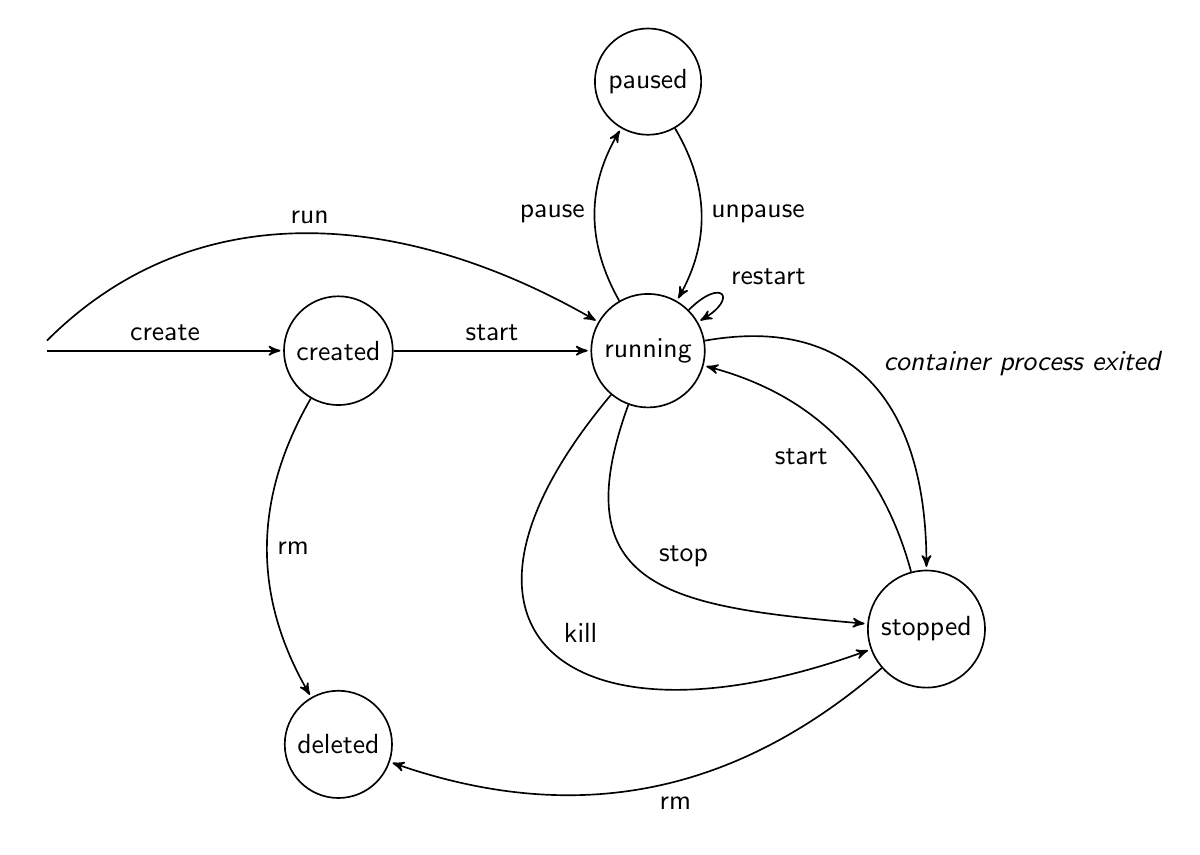
\begin{tikzpicture}[->,>=stealth',shorten >=1pt,auto,node distance=5cm, semithick]
        \sffamily\fontsize{10}{10}\selectfont
        \node (cr){};
        \node (run){};
        \node[state] (A)     [right =3cm of cr]         {created};
        \node[state]         (B) [right =2.5cm of A] {running};
        \node[state]         (C) [below right of=B] {stopped};
        \node[state]         (D) [above =2cm of B] {paused};
        \node[state]         (E) [below of=A] {deleted};

        \path (cr) edge [] node {create} (A)
            (run) edge [out=45,in=150]                     node {run} (B)
              (A) edge []                              node {start} (B)
                  edge [bend right]                    node {rm}    (E)
              (B) edge [out=230, in=200, distance=4cm] node {kill}  (C)
                  edge [out=250,in=175, distance=2.5cm]node {stop}  (C)
                  edge [bend left]                     node {pause}  (D)
                  edge [in=30, out=45, loop]           node {restart}  (D)
                  edge [out=10, in=90, distance=2cm]   node {\textit{container process exited}}  (C)
              (C) edge [bend right]                    node {start}  (B)
                  edge [bend left]                     node {rm}  (E)
              (D) edge [bend left]                     node {unpause} (B)
              ;
      \end{tikzpicture}
      \caption*{Simplified version. Commands should be understood prefixed with \textit{docker}. \newline \scriptsize Based on https://docs.docker.com/engine/reference/api/docker\_remote\_api/\#docker-events }
      \caption[Docker Container Life Cycle]{Docker Container Life Cycle \cite{Docker2016Docker}}
      \label{fig:docker_container_lifecycle}
    \end{figure}

    One possible variation on $G_{1C}^{DV}$ and $G_{SEPC}^{DV}$ would be the inclusion of engine logic in the workflow instance container. While the scheduling of this container and preparations on the targeted node would still be in the responsiblity of the main \acp{WfMS}' workflow engine, the control over the started activity instances would be handed to a smaller, workflow instance specific engine.
    This setup facilitates the management of the required directory structure, since the container that issues the commands has direct access to the data volume.

    Further, suspending and resuming of workflows and activities could both be realized with the respective pause/unpause Docker commands. In combination with a checkpoint/restore tool, which provides the means to save and restore the memory state of a process, long running workflows could be paused and restored across server restarts, or be migrated to another server, if necessary. Proofs of concept for the feasibility of this procedure have been presented in the past \cite{Kim2015Checkpoint,Merker2015How}.

    A drawback of this variation is, that the status of the enactment is then held in the workflow instance container. By following the event stream, started and stopped activity instances could be tracked by the main workflow engine, but low-level details would have to be transferred separately, if it was needed there.
  % subsubsection element_wrapping_containers (end)

  \subsubsection{Worker Containers} % (fold)
  \label{ssub:worker_containers}
    The $*_{WORK}^{*}$ variants take a different approach at utilizing Docker for workflow enactment, in which many unspecialized containers are running constantly. These containers, when provided with an activity description and input data, perform the required actions and return to a waiting state until they are provided with a task again.

    Opposed to the variant presented in \ref{ssub:element_wrapping_containers}, there is no one-to-one correlation of an image to an activity or a workflow, and also none of a container to an activity instance or a workflow instance. Hence, there is no further creation and distribution of images required -- besides the initial distribution of the workers' images (and, eventually, invoked third-party images).
    Since all information that is required for execution is passed to these workers at each invocation, changes to definitions of activities or workflows may immediately show effects. This flexibility comes at the price of a verbose communication, though.

    Another benefit of worker containers is that they facilitate swift adaption to workload peaks. In case that scheduled enactments start to accumulate, more worker containers may be run. If the nodes themselves have reached their resource limitations, new nodes may be added to the swarm, which do not have to be provisioned with all activity or workflow images -- as it would be the case with the wrapping-images variant -- but rather only with the worker image.
  % subsubsection worker_containers (end)

  \subsubsection{Data Exchange via Data Volume} % (fold)
  \label{ssub:data_exchange_via_data_volume}
    The idea behind this concept ($*_{*}^{DV}$) is, that all containers involved in the execution of one workflow instance have access to a common working directory, in which the data visibility scopes can be established using a file system structure. This working directory resides in a data volume owned by a container that belongs exclusively to the respective workflow instance and whose only purpose is to ensure the existence of said volume.

    % - data volume mountable via -v option
    % - arbitrary name and location in container

    In its simplest form the working directory could be a simple shared directory, which is managed cooperatively by all related containers. Activity instances could then read and write files to that directory.
    \textcolor{red}{**PRO/CON?**}

    A more elaborate structure could be imposed on the working directory, too. In order to support the data visibility and data interaction types that were chosen in \ref{ssub:workflow_execution}, the following directory structure could be used, which is depicted in Figure~\ref{fig:dv_dir_structure}.
    Data defined at build time, \ie environment data, workflow data and activity data, could each be stored in a separate subdirectory of the main working directory \texttt{workflow\_relevant\_data}. The directories for workflow data and activity data should have uniquely identifyiable names that can be infered from the respective workflow element, \eg \texttt{wf\_\$workflow\_id} and \texttt{ac\_\$activity\_id}. Data that is shared among multiple instances of one activity could be stored in a subdirectory \texttt{shared} of the respective activity data directory.

    Also present in the working directory should be a directory \texttt{wfi\_\$workflow\_instance\_id}, in which the working directories for subsequently started activity instances and workflow instances can be stored. Each activity instance is then assigned a directory \texttt{aci\_\$activity\\\_instance\_id} within that that working directory. In case that the activity instance in question is a sub-workflow activity, the respective workflow instance's working directory resides in the sub-workflow activity instance's working directory. This principle can then be repeated recursively, as visible in Figure~\ref{fig:dv_dir_structure}.

    Depending on the desired level of isolation, the instance containers could be instructed to mount either a) the whole \texttt{workflow\_relevant\_data} directory or b) just their own working directory, the directories that contain the data defined at build time, and working directories of activity or workflow instances which they were configured to use. While the former is a much simpler solution, the latter gives more fine-grained control over the data that each instance is allowed to access.

    \begin{figure}[htbp]
      \centering
      \begin{forest}
        dir tree
        [workflow\_relevant\_data
          [env]
          [wf\_1cc594ba-...]
          [wf\_b45d2564-...]
          [ac\_0225d86f-...
            [shared]
          ]
          [ac\_2a5aa4ff-...]
          [ac\_7fc09132-...]
          [wfi\_e65c8533-... \textcolor{gray}{(instance of wf\_1cc594ba-...)}
            [aci\_76b8680c-... \textcolor{gray}{(instance of ac\_0225d86f-...)}]
            [aci\_1e09d287-... \textcolor{gray}{(instance of ac\_2a5aa4ff-...)}
              [wfi\_68e17268-... \textcolor{gray}{(instance of wf\_b45d2564-...)}
                [aci\_2708fd1a-... \textcolor{gray}{(instance of ac\_7fc09132-...)}]
              ]
            ]
          ]
        ]
      \end{forest}
      \caption{Exemplary directory structure for $G_{*}^{DV}$}
      \label{fig:dv_dir_structure}
    \end{figure}


    $G_{*}^{DV}$ natively supports all identified types of data visibility by providing respective directories and access to them, with the limitation that workflow data and environment data has to be copied to the data volume before execution and is thus restricted to the state it had at that time. Altering this data is possible, \eg by replacing the respective files via \texttt{docker copy} or altering it in a \texttt{docker exec} session, but extra measures have to be taken to request such an up-to-date version.

    Data interactions between activity instances, a sub-workflow activity and its related components and vice versa are supported by $G_{*}^{DV}$. Exchanging data between two running workflow instances is not possible on this way, since mounting volumes to running containers is not supported by Docker yet. This kind of interaction thus requires some additional tools. It would be possible to grant access to workflow instances running on the same machine -- at the price of loss of control over data visibility -- by mounting the top-level working directory of that machine in all containers.

    As long as no requests to external sources are made within the workflow, data has to be transferred over the network only twice in this approach -- for the input and output of the workflow instance. All subsequent data transfers are either implicit, \eg by accessing the respective working directory or a symbolic link to it, or take place on the local machine, \eg copying one or more files. Because of transfer rates *QUOTE*, $G_{*}^{DV}$ has an advantage over message-based approaches when it comes to processing of large and/or many data sets, \ie log files, genome research data or images. Also, unless required by the activities themselves, data conversion is less of an issue since relying on the file system allows arbitrary file types to be used.

    Sharing a data volume using only Docker tools requires all containers to be on the same machine, which is why there is no spread version $S_{*}^{DV}$ of this concept. Approaches exist to utilize \ac{NFS} or \ac{P2P} file sharing for distributed access to data volumes, but given the limited scope of this thesis they shall not be regarded further here \cite{Miell2015How}.

    $G_{1C}^{DV}$ could theoretically work on its own file system in the editable layer of the container without a dedicated data volume, since all workflow components would have access to it. This would make the container self contained on the one hand -- and thus easier to export or migrate -- but would on the other hand couple the data life cycle to the processing container's life cycle. That is, if the container is removed, the data is removed with it.

    In order for $G_{WORK}^{DV}$ to work successfully, it is inevitable that only workers on the same node as the data volume are used for the workflow enactment, since workers on different nodes could not access that data volume.
  % subsubsection data_exchange_via_data_volume (end)

  \subsubsection{Data Exchange via Service} % (fold)
  \label{ssub:data_exchange_via_service}
    $*_{*}^{SER}$ represents the concept of providing some service that is able to store and serve workflow relevant data on request. This implies, that the instance containers have to feature a mechanism to communicate to this service.

    The data-providing service could either be running as a single instance on some node in the network or on each node in the network. While the former avoids having to deal with synchronization between service instances and inconsistencies resulting from race conditions, the latter could balance the load. (shorten response times? hops)

    Since the storage of workflow related data is decoupled from the execution in $*_{*}^{SER}$, the coverage of data visibility and data interaction capabilities depends on the chosen underlying service. Theoretically, all forms of data visibility and interactions should thus be possible. Also, the solution exhibits the same properties for grouped and spread execution alike, for the same reason.

    In this variant, data is transferred before and after each step in the workflow, \ie when the execution starts, when it ends, whenever an activity is instantiated or an instance finished its work. This is only economical if the amount of data is sufficiently small or if the workflows consist of few activities. In order for the workflow execution to function correctly, the data management service must be reliably available to all containers.
  % subsubsection data_exchange_via_service (end)

  \subsubsection{Data Exchange via Direct Communication} % (fold)
  \label{ssub:data_exchange_via_direct_communication}
    In this scenario, the containers communicate with each other directly in order to exchange workflow relevant data. It can be split again in two sub-variants, according to the data passing patterns noted in \ref{sub:workflow_data}. On the one hand, one where the workflow relevant data is passed along the control flow ($*_{*}^{D_a}$). On the other hand, one where containers can query each other for their data($*_{*}^{D_b}$).

    In $*_{*}^{D_a}$, the data flow is is directly coupled to the control flow, \ie all data is passed on on invocation. This requires all data that might be used in another activity instance to be passed along, no matter whether the succeeding activity uses them or not \cite{Russell2005Workflow}. While this variant allows to pass (and update) workflow and environment data, it may be problematic for larger amounts of data.

    $*_{*}^{D_b}$ requires all containers that shall be queried for data to provide some communication mechanism and to be running. Thus, in the worst case every container related to the workflow instance in question has to be kept running. Even though the containers' use of processor time can be reduced by pausing them until they are needed, this approach could impose a considerable strain on the host machine's memory, as pausing containers has no effect on their memory consumption.
    Workflow data and environment data in $*_{*}^{D_b}$ may be provided to the first activity, which then could be queried for a (static) version of it.

    Because workflow instances are not represented as containers in $*_{AC}^{D}$, $*_{AC}^{D_b}$ provides no means to store and access sub-workflow data, multiple instance data and workflow instance data.

    $*_{WORK}^{D_b}$ is no useful solution, as keeping the worker containers occupied with one activity in order to make them queryable would block their use for other workflow instances, thus rendering the \ac{WfMS} incapable of processing further workflow instances once all workers are invoked -- unless further workers are spawned.

    As all workflow components reside in one container in $G_{1C}^{D}$, no communication between containers is necessary -- all data can be exchanged on an arbitrary way within that single container. This variant thus represents a special case.
  % subsubsection data_exchange_via_direct_communication (end)
% subsection mode_of_operation_of_the_aspects (end)

\begin{table}[!htbp]
  \centering
  %\renewcommand*{\arraystretch}{1.7}
  \begin{tabular}{C{1cm} C{1cm} C{1cm} C{1cm} C{1cm} C{1cm} C{1cm} | C{1cm} C{1cm} C{1cm} C{1cm}}
    \toprule

    \multicolumn{6}{c}{Data Visibility} & \multicolumn{4}{c}{Data Interactions} \\

      & \rot{Ac Data}
      & \rot{SubWF Ac Data}
      & \rot{MultInst Ac Data}
      & \rot{WFInst Data}
      & \rot{WF Data}
      & \rot{Env Data}

      & \rot{Ac $\rightarrow$ Ac}
      & \rot{SubWF Ac $\rightarrow$ SubWF}
      & \rot{SubWF $\rightarrow$ SubWF Ac}
      & \rot{WFInst $\rightarrow$ WFInst}
    \\ \midrule

    $G_{AC}^{DV}$    & \ja     & \ja              & \ja              & \ja              & \ja ($\dagger$) & \ja ($\dagger$) & \ja              & \ja              & \ja              & $\bigcirc$      \\ \midrule
    $G_{SEPC}^{DV}$  & \ja     & \ja              & \ja              & \ja              & \ja ($\dagger$) & \ja ($\dagger$) & \ja              & \ja              & \ja              & $\bigcirc$      \\ \midrule
    $G_{1C}^{DV}$    & \ja     & \ja              & \ja              & \ja              & \ja ($\dagger$) & \ja ($\dagger$) & \ja              & \ja              & \ja              & $\bigcirc$      \\ \midrule
    $G_{WORK}^{DV}$  & \ja     & \ja              & \ja              & \ja              & \ja ($\dagger$) & \ja ($\dagger$) & \ja              & \ja              & \ja              & $\bigcirc$      \\ \midrule

    $G_{AC}^{SER}$   & \ja     & \ja              & \ja              & \ja              & \ja             & \ja             & \ja              & \ja              & \ja              & \ja             \\ \midrule
    $G_{SEPC}^{SER}$ & \ja     & \ja              & \ja              & \ja              & \ja             & \ja             & \ja              & \ja              & \ja              & \ja             \\ \midrule
    $G_{1C}^{SER}$   & \ja     & \ja              & \ja              & \ja              & \ja             & \ja             & \ja              & \ja              & \ja              & \ja             \\ \midrule
    $G_{WORK}^{SER}$ & \ja     & \ja              & \ja              & \ja              & \ja             & \ja             & \ja              & \ja              & \ja              & \ja             \\ \midrule

    $G_{AC}^{D_a}$   & \ja     & \ja              & $\bigcirc$       & \ja              & \ja             & \ja             & \ja ($\ddagger$) & $\bigcirc$       & $\bigcirc$       & $\bigcirc$      \\ \midrule
    $G_{AC}^{D_b}$   & \ja     & $\bigcirc$       & $\bigcirc$       & $\bigcirc$       & $\bigcirc$      & $\bigcirc$      & \ja ($\ddagger$) & $\bigcirc$       & $\bigcirc$       & $\bigcirc$      \\ \midrule
    $G_{SEPC}^{D}$   & \ja     & \ja ($\ddagger$) & \ja ($\ddagger$) & \ja ($\ddagger$) & $\bigcirc$      & $\bigcirc$      & \ja ($\ddagger$) & \ja ($\ddagger$) & \ja ($\ddagger$) & \ja ($\ddagger$)\\ \midrule
    $G_{1C}^{D}$     & \ja$^*$ & \ja$^*$          & \ja$^*$          & \ja$^*$          & $\bigcirc$      & $\bigcirc$      & \ja$^*$          & \ja$^*$          & \ja$^*$          & \ja$^*$         \\ \midrule
    $G_{WORK}^{D}$   & \ja     & \ja ($\ddagger$) & \ja ($\ddagger$) & \ja ($\ddagger$) & $\bigcirc$      & $\bigcirc$      & \ja ($\ddagger$) & \ja ($\ddagger$) & \ja ($\ddagger$) & \ja ($\ddagger$)\\ \midrule

    $S_{AC}^{SER}$   & \ja     & \ja              & \ja              & \ja              & \ja             & \ja             & \ja              & \ja              & \ja              & \ja             \\ \midrule
    $S_{SEPC}^{SER}$ & \ja     & \ja              & \ja              & \ja              & \ja             & \ja             & \ja              & \ja              & \ja              & \ja             \\ \midrule
    $S_{WORK}^{SER}$ & \ja     & \ja              & \ja              & \ja              & \ja             & \ja             & \ja              & \ja              & \ja              & \ja             \\ \midrule

    $S_{AC}^{D}$     & \ja     & $\bigcirc$       & $\bigcirc$       &  $\bigcirc$      & $\bigcirc$ & $\bigcirc$  & \ja ($\ddagger$) & $\bigcirc$       & $\bigcirc$       & $\bigcirc$      \\ \midrule
    $S_{SEPC}^{D}$   & \ja     & \ja              & \ja              & \ja              & $\bigcirc$ & $\bigcirc$  & \ja ($\ddagger$) &\ja ($\ddagger$)  & \ja ($\ddagger$) &\ja ($\ddagger$) \\ \midrule
    $S_{WORK}^{D}$   & \ja     & \ja              & \ja              & \ja              & $\bigcirc$ & $\bigcirc$  & \ja ($\ddagger$) &\ja ($\ddagger$)  & \ja ($\ddagger$) &\ja ($\ddagger$) \\ \bottomrule
  \end{tabular}
  \captionsetup{justification=centering}
  \caption*{\ja~ natively supported ~~|~~ \ja$^*$~ natively supported, a direct connection within the container is assumed ~~|~~ \ja ($\dagger$)~ can be passsed on instantiation, real-time access requires additional tools \\ \ja ($\ddagger$) natively supported, assuming that all containers are left running for the time of workflow execution ~~|~~ $\bigcirc$~ not natively supported, requires additional tools \\[1em]

  Ac = Activity ~|~ SubWF = Sub-workflow~|~ MultInst = Multiple instance ~|~ WFInst = Workflow instance~|~ WF = Workflow ~|~ Env = Environment
  }
  \label{tab:docker_variants}
  \caption{Containerization/Grouping/Communication Solution Pairings}
\end{table}

\subsection{Identification of promising combinations} % (fold)
\label{sub:promising_combinations_of_characteristics}
  Due to its shortcomings regarding the supported types of data visibility and interactions, direct communication between instance-related containers ($*_{*}^{D}$) is ruled out as a candidate for the prototype. The remaining combinations may be eligible depending on the intended use case and desired properties of the \ac{WfMS}, \eg the kind of data that is processed, the targeted infrastructure, and nature of the workflows.

  If the data volume approach is chosen, one is committed to grouped execution on one node. Considering the different containerization solutions, $G_{SEPC}^{DV}$ is favorable over $G_{AC}^{DV}$, because the explicit existence of containers which represent (sub-)workflow instances makes it possible to both track their state using Docker mechanisms and manage their respective working directories. Embedding workflow engine logic into these containers could enable workflows to be exported and used in a stand-alone fashion.

  $G_{SEPC}^{DV}$ is also favorable over $G_{1C}^{DV}$ for general use, because the modularity of $G_{SEPC}^{DV}$ permits to update single activities within the workflow by distributing new versions of their respective image. In $G_{1C}^{DV}$, the whole image would have to be updated due to the way layering in Docker images works. Also, $G_{1C}^{DV}$ does not provide the means to track the activity instances' life cycles with Docker mechanisms, only that of the workflow instance. If the workflow is not meant to be updated but to be distributed to third parties as a stand-alone solution, \eg an automated batch process for photos, which is sold to photographers, this variant could be a viable option, however.

  The main benefit of $*_{WORK}^{*}$ is that it allows to distribute the workload among several workers. Since $G_{*}^{DV}$ requires all involved workers to be on the same machine, this advantage is void for the combination $G_{WORK}^{DV}$.

  Altogether, this makes $G_{SEPC}^{DV}$ the variant of choice for data-intense use cases.

  When comparing the service-based variants with each other, $G_{*}^{SER}$ and $S_{*}^{SER}$ share most their advantages and drawbacks. $S_{*}^{SER}$ permits the containers to run on different nodes, though. As this allows containers to be assigned to machines according to their resource requirements and the momentary workload of a machine, it is the preferred variant of those two.

  Because the decoupling of data and containers is well supported by $*_{*}^{SER}$, it is a good fit for the worker-based approach of $*_{WORK}^{*}$, which in turn facilitates load balancing. A use case for $S_{WORK}^{SER}$ could be \ac{WfMS} users like market research companies, which create lots of frequently updated form-centric workflows for call center agents to use, \ie fast-changing workflows with rather small data that has to be passed.

  The results of the above reasoning are roughly summarized in a decision tree in Figure~\ref{fig:choosing_docker_utilization}, which is intended to give a hint on the suitable utilization of Docker for workflow enactment for a given use case.

  \begin{figure}[htbp]
    \centering
    \newdimen\nodeDist
    \nodeDist=35mm
    \begin{tikzpicture}[
        node/.style={%
          draw,
          rectangle,
        },
      ]

        \node [align=center, node] (A) {Focus on standalone execution \\of workflows?};
        \path (A) ++(-135:\nodeDist) node [align=center, node] (B) {$G_{1C}^{DV}$};
        \path (A) ++(-45:\nodeDist) node [align=center, node] (C) {Expected data size};
        \path (C) ++(-135:\nodeDist) node [align=center, node] (D) {$G_{SEPC}^{DV}$};
        \path (C) ++(-45:\nodeDist) node [align=center, node] (E) {Expected change rate of \\ activities/process definitions};
        \path (E) ++(-45:\nodeDist) node [align=center, node] (F) {$S_{WORK}^{SER}$};
        \path (E) ++(-135:\nodeDist) node [align=center, node] (G) {$S_{AC/SEPC}^{SER}$};

        \draw (A) -- (B) node [left,pos=0.5] {yes}(A);
        \draw (A) -- (C) node [right,pos=0.5] {no}(A);
        \draw (C) -- (D) node [left,pos=0.5] {large}(A);
        \draw (C) -- (E) node [right,pos=0.5] {smaller}(A);
        \draw (E) -- (F) node [right,pos=0.5] {frequent}(A);
        \draw (E) -- (G) node [left,pos=0.5] {seldom}(A);
    \end{tikzpicture}
    \caption{Choosing the right utilization of Docker for workflow enactment}
    \label{fig:choosing_docker_utilization}
  \end{figure}
% subsection promising_combinations_of_characteristics (end)

\subsection{Utilization of third-party images} % (fold)
\label{sub:execution_of_third_party_containers}
  The motivation behind enabling the use of third-party images is that theoretically, any program which is able to run in a Docker container may be incorporated in a workflow this way. In 2015, over 125.000 public repositories existed \cite{Dehamer2015Docker}.

  Before these images can be used by a workflow instance, they have to be present on the node that they will be run on. The provision of nodes with the required images could either happen actively, thus qualifying the node for the execution of said image, or passively, \ie the node is selected for running the image in question and fetches it in the course of running it. While the the former solution limits the number of nodes that are able to run the image -- unless every node is provisioned with it -- the latter solution is likely to delay the enactment of the workflow at its first use for the time it takes to pull the respective image.

  As third-party images are likely to be unaware of their utilization in a workflow, it is not guaranteed that their output suits the needs of the \ac{WfMS}. Also, these images may require some parametrization for their instantiation. On the one hand, both issues could be approached by the workflow engine, which might transform the output and provide suitable parameters based on the activity's configuration. On the other hand, an utility activity could be introduced that can be configured such that it is able to instantiate the third-party image and transform its output to a suitable format.
  The latter solution should be preferred, as it shifts the responsibility for the aforementioned tasks away from the workflow engine, which reduces the engine's complexity. The engine does not need to differentiate between custom and foreign images in this case.

  \textcolor{red}{**Argumentation schwach**}

  In order to be able to instantiate the third-party image, the adapter image requires access to its host node's Docker daemon.
% subsection execution_of_third_party_containers (end)


\subsection{Execution Scheduling} % (fold)
\label{sub:execution_scheduling}
  In the course of a workflow enactment, several containers have to be instantiated -- unless the worker-based approach ($*_{WORK}^{*}$) is chosen. Choosing the node on which the instantiation takes place is a task that may impact the performance of the containers and the enactment itself, as the nodes may differ regarding their available resources. It is thus of interest to examine by which rules or criteria the scheduling may take place and whether and how the user should be able to take influence on the scheduling.

  \subsubsection{Scheduling Abilities of Docker Swarm} % (fold)
    \label{ssub:abilities_of_docker_swarm}
    As mentioned in \ref{sub:docker_swarm}, Docker Swarm offers two kinds of scheduling mechanisms: filters and strategies. Filters can be passed on instantiation as an environment variable parameter with the format \texttt{<filter-type>:<key><operator><value>}. The value of \texttt{filter-type} can either be ``constraint'' or ``affinity'' -- the two types of filters supported by Swarm.

    \texttt{<key>} can take the values \emph{node} or \emph{container} (which signals a comparison to the respective name or \ac{ID}), one of the default node tags, or the name of some custom label which can refer to both node labels and container labels. By default, nodes get tagged by Docker with a name, their \ac{ID}, their storage driver, their execution driver, the kernel version they use and the name of their operating system.
    Custom labels may be applied to nodes when their daemon is started and to containers as a parameter to the \texttt{run} command. In order to avoid conflicting label names, reverse domain name notation is advised by Docker.
    \texttt{<operator>} may either take the value \texttt{==} or \texttt{!=}, indicating whether a match is desired or should be avoided. It can be followed by a tilde, \eg \texttt{==~} to signal that if the condition cannot be met, the container should be scheduled according to a strategy instead.
    The \texttt{<value>} is a string made of alpha-numeric characters, dots, hyphens, and underscores. It may be either a regular expression or a globbing pattern, to which names, \acp{ID} tags or labels will be matched against.

    Constraints focus on the characteristics of nodes for scheduling; either \ref{itm:const_first} some identifier or \ref{itm:const_second} node tags or \ref{itm:const_third} labels:

    \begin{enumerate}[label=\alph*), nosep]
      \item \label{itm:const_first} \texttt{constraint:node==...}
      \item \label{itm:const_second} \texttt{constraint:operatingsystem==...}
      \item \label{itm:const_third} \texttt{constraint:com.example.label==...}
    \end{enumerate}

    Affinities can be specified to schedule containers based on the presence of images or containers on the target node. Possible criteria are \ref{itm:aff_first} container names or \acp{ID}, \ref{itm:aff_second} image names or \acp{ID} or \ref{itm:aff_third} a custom label on a container:

    \begin{enumerate}[label=\alph*), nosep]
      \item \label{itm:aff_first} \texttt{affinity:container==...}
      \item \label{itm:aff_second} \texttt{affinity:image==...}
      \item \label{itm:aff_third} \texttt{affinity:com.example.label==...}
    \end{enumerate}

    Further, there are some implicit forms of scheduling. First, containers will not be executed on nodes that Swarm considers \emph{unhealthy}, \ie that do not respond or otherwise exhibit faulty behavior. Second, some Docker features imply scheduling rules. If the container requires an exposed port, it will not be scheduled on nodes where this port is already occupied. Mounted volumes of, a shared network stack with or a link to another container imply an affinity to that container, which will prohibit the execution if it is not met.
  % subsubsection abilities_of_docker_swarm (end)

  \subsubsection{Identification of Possible Scheduling Criteria} % (fold)
  \label{ssub:identification_of_desired_scheduling_criteria}
    In order to examine scheduling solutions, some goals should be specified to which they can be evaluated against -- an exhaustive list of these goals is not in the scope of this thesis, though. Thus, two groups of exemplary scheduling criteria are considered, which are depicted in Table~\ref{tab:scheduling_criteria}.

    On the one hand, scheduling may be performed based on the properties of the nodes, which can be of qualitative or quantitative nature, their tags or the execution environment they have to offer. Examples for qualitative node properties could be its name, present containers or images, geographical location, the nature of its storage device, or its membership in some arbitrary groups. Quantitative properties of interest might be the amount of available memory or storage, the number of currently running containers or the node's network speed.

    On the other hand, containers may be assigned to nodes based on \ac{WfMS}-specific data. This could be for example properties of the underlying activities and workflows, the status and data of their instances or the state of a custom scheduling mechanism of the \ac{WfMS}. For example, if an user specifies his/her current location in the course of a workflow enactment, all subsequent containers could be scheduled to run on nodes that suit the laws of that country.

    \begin{table}[!htbp]
      \centering
      \begin{tabular}{l l l}
        \toprule
        Data Source & Criterion Type & Examples \\
        \midrule
        Docker
          & Node tags
            & Name \\
            && \ac{ID} \\
            && Storage driver \\
            && Execution driver \\
            && Kernel version  \\
            && Operating system \\ [1.2ex]
          & Qualitative node properties
            & Geographic location\\
            && Custom grouping membership\\
            && Ownership status\\ [1.2ex]
          & Quantitative node properties
            & Available memory \\
            && Available storage \\
            && Network speed \\ [1.2ex]
          & Execution environment
            & Existing containers \\
            && Existing images \\
            && Currently running containers \\ [1.4ex]
        WfMS
          & Live data
            & Enactment status \\
            & Activity input/output data \\
            && Workflow input/output data \\ [1.2ex]
          & Activity/workflow properties
            & Expected data-intensity \\
            && Compliance requirements\\
            &&\\ [1.2ex]
        \bottomrule
      \end{tabular}
      \label{tab:scheduling_criteria}
      \caption{Scheduling Criteria}
    \end{table}

    Both qualitative and quantitative properties of a node can be stored in custom labels on that node.
    Qualitative values can simply be stored as strings and used in constraints via globbing and regular expressions. Assuming, for example, the nodes had their location stored as a label with the format

    \centerline{\texttt{com.example.location=\$country}}

    with \texttt{\$country} being the respective ISO 3166-1 alpha-2 code \cite{Standardization2013De}; and the information whether they belong to the own company or are rented servers stored as a label with the format

    \centerline{\texttt{com.example.internal=\$internal}}

    with \texttt{\$internal} being the string representation of a boolean value. Then, in order to schedule a container to a self-owned node in Germany running any version of the \emph{Ubuntu} operating system, the following combination of tag and label constraints could be used:

    \centerline{\texttt{constraint:operatingsystem==Ubuntu*}}
    \centerline{\texttt{constraint:com.example.location==de}}
    \centerline{\texttt{constraint:com.example.internal==true}}

    Quantitative values stored in a label may be queried with comparisons using regular expressions. Assuming all nodes have a label that specifies their amount of memory, which has the form

    \centerline{\texttt{com.example.ram=\$mem}}

    with \texttt{\$mem} being the amount of memory in megabytes. In this setting, a container can be scheduled to a node with at least 650 megabytes of memory by enforcing the constraint

    \centerline{\texttt{constraint:com.example.ram==/([6][5-9]{\textbackslash}d|[7-9]{\textbackslash}d\{2,\}|{\textbackslash}d\{4,\})/}.}

    This regular expression will match a) any number with four or more digits and b) any three digits number that starts with a number in the range of 7-9 and c) any three digits number that starts with 6 and continues with a number in the range of 5-9. Analogously to this, other quantitative measures may be stored and queried.

    Scheduling constraints regarding present images and containers can be realized using the appropriate affinity filters. One possible use case is to ensure, that all images and containers required for the enactment of a workflow element are present:

    \centerline{\texttt{affinity:image==required-image-name}}
    \centerline{\texttt{affinity:container==required-container-name}}

    At the current state of Docker Swarm, it is not possible to make sure that the containers are not only present but also running. If it is required, this criterion has to be addressed by some custom mechanism of the \ac{WfMS}, \eg a method that queries the swarm master's \ac{API}, selects a suitable node with running instances of the required container and constructs an according node constraint.

    Since updating labels and tags of containers and nodes after their creation is not possible at the time of writing, all \ac{WfMS} related data created during enactment has to be sent to the system and managed internally by it.

    Properties of activities and workflows that has been defined at build time may be stored in the form of labels when they are created. This is possible by using the \texttt{LABEL} command for desired labels in the respective Dockerfile in combination with passing their value as an argument for the build command:

    \textcolor{gray}{in Dockerfile:}

    \centerline{\texttt{\textbf{LABEL} com.example.expected-data-intensity=\$data-intensity}}

    \textcolor{gray}{in command line:}

    \centerline{\texttt{docker build [...] --build-arg data-intensity=high [...]}}

    In contrast to other examples given in this thesis, \texttt{\$data-intensity} should not be understood as a placeholder, as it is the actual Dockerfile syntax for the interpolation of a passed build argument with the respective name.

    The workflow engine could then use the image's labels to take the stored properties into account for scheduling. For complex properties, labels containing serialized JSON objects could be used \cite{Docker????Docker}.
  % subsubsection approaches_for_scheduling_criteria (end)

  \subsubsection{Implications of Other Design Decisions} % (fold)
  \label{ssub:implications_of_other_design_decisions}
    \acp{WfMS} may let the workflow modeling developer take influence on the scheduling of workflow containers by letting that user define constraints or affinities on them at build time. This could be beneficial because of the user's potential a priori knowledge on these elements, \eg whether they are data-intensive and thus require some large storage, or because it enables meeting compliance rules, \eg concerning the geographical location of data storage and processing.

    Since the $G_{*}^{DV}$ approaches are grouped on one node by definition, the scheduling takes place for the first container only, while subsequent containers are bound to the same node by the implicit affinity created through the mounted data volume.

    There is no need for scheduling in the sense of managing container startups in the $*_{WORK}^{*}$ use case, since the workers are already running. One could impose restrictions on the set of workers that are allowed to work on a task, though.
  % subsubsection implications_of_other_design_decisions (end)
% subsection execution_scheduling (end)

      % section docker_for_wf_execution (end)

    \section{System Architecture} % (fold)
      \label{sec:architecture}

      With the objectives determined in Section \ref{sec:determination_of_objectives} in mind, a Docker-based architecture is developed in this section. First, possible architecture styles are presented in \ref{sub:application_structure}, of which one is then chosen with regards to potential benefits in combination with Docker. Subsequently, the manner users interact with the system is chosen in \ref{sub:user_interaction_with_the_system} and the high-level mode of communication between containers in \ref{sub:inter_component_communication}.

      % -*- root: ../../main.tex -*- %

\subsection{Application Structure} % (fold)
  \label{sub:application_structure}
  Micro-services, service discovery \cite{Stubbs2015Distributed}

  Use Docker only for execution vs docker all the things

  Developers of software systems have to cope with factors which impose challenges on them, such as high complexity within their systems, an increased need for integration of internal and external functionality and evolving technologies. Several architectural approaches emerged from the attempt to overcome these challenges. Strîmbei et al consider \emph{monolithic architecture}, \emph{\ac{SOA}} and \emph{Micro-services} to be the most relevant \cite[p.~13]{Strimbei2015Software}.

  \paragraph{Monolithic Architecture} % (fold)
    \label{par:monolithic_architecture}
    Monolithic software systems are characterized by their cohesive structure. Usually, components in a monolith are organized within one programm, often running in one process \cite[p.~35]{Stubbs2015Distributed}. They communicate through shared memory and direct function calls. Monolithic applications are typically written using one programming language \cite[p.~14]{Strimbei2015Software}. In order to cope with increasing workload on a monolithic system, multiple instances of it are run behind a load balancer \cite[p.~35]{Stubbs2015Distributed}.

    The strengths of monolithic architecture lie mostly in its comparably simple demands towards the infrastructure. As the application is run as one entity, deployment and networking are rather simple \cite[p.~35]{Stubbs2015Distributed}. Since data can be shared via memory or disk, monolithic applications can access it faster than it would be the case with networked components \cite[p.~14]{Strimbei2015Software}. \\
    Also, as the interaction between the application's components happens XYZ, the complexity of this interaction is lower compared to interaction between distributed components \cite[p.~14]{Strimbei2015Software}.

    The weaknesses of monolithic architecture stem from its cohesive nature. As its components are usually tightly coupled, changes to one component can affect other parts of the application, which complicates the introduction of new components and the refactoring of existing ones \cite{Stubbs2015Distributed}.
    Components cannot be deployed individually, which hinders reuse of functionality across several applications more difficult and makes scaling of single bootleneck components impossible \cite{Stubbs2015Distributed}. Also, if the application runs in a single process, the failure of one component may bring down the whole application \cite[p.~5]{Newman2015Building}.

    In combination with Docker, a possible solution could look like this: ...
    % paragraph monolithic_architecture (end)

  \paragraph{Service-oriented Architecture} % (fold)
    \label{par:service_oriented_architecture}
    \ac{SOA} is based on the idea that code which provides related business functions can be bundled into one component which offers said functionality to other systems \emph{as a service}, thus avoiding duplicated implementation of the functionalities among these systems \cite[p.8]{Hohpe2004Enterprise}.
    An application may then use several services in order to fulfill its own business function \cite[p.~390]{Papazoglou2007Service}.
    The \ac{OASIS} describes \ac{SOA} as an architectural paradigm that supports the organization and usage of these services \cite{Standards2006Reference}. Each service provider exposes its offered services in a standardized way, \eg using \ac{WSDL}, which can then be utilized by \emph{service consumers} \cite[p.~390]{Papazoglou2007Service}, \cite[p.~17]{Strimbei2015Software}.

    Messages between services in \ac{SOA} are either of direct nature, which is called point-to-point connection, or backed by a message bus, the \ac{ESB} which incorporates the integration logic, \eg on transport and transformation of messages, between services and supports asynchronous messages \cite[p.~393]{Papazoglou2007Service}. While the former leads to tight coupling between the components, which becomes impractical with increasing numbers of endpoints, the latter manages this scenario better \cite[p.~393]{Papazoglou2007Service}.

    On the one hand, \ac{SOA} has some advantages in comparison to monolithic architecture.
    Service consumers do not have to make assumptions - or know - how services work, they only have to rely on the invokation of a service and its result to be formed as expected \cite[p.~390]{Papazoglou2007Service}. As long as the interface and the output of existing services do not change, a service provider may thus be altered or its capabilities be extended without affecting its services' consumers \cite[p.~390]{Papazoglou2007Service}. \ac{SOA} thus enhances an organization’s ability to respond quickly to changes \cite[p.~390]{Papazoglou2007Service}, \cite[p.~254]{Choi2010Implementing}. \\
    Since legacy applications can be provided with appropriate interfaces, SOA can help to integrate and extend them \cite[p.~390]{Papazoglou2007Service}.

    On the other hand, \ac{SOA} has some drawbacks, too.
    For example, the failure of a single service provider may bring down multiple applications that consume its services, if no fallback measures are in place \cite[p.~408f]{Papazoglou2007Service}.
    Also, the overall performance of an application with \ac{SOA} depends on the aggregated performances of the services it uses and their respective interactions \cite[p.~408f]{Papazoglou2007Service}.

    In combination with Docker, a possible solution could look like this: ...
    % paragraph service_oriented_architecture (end)

  \paragraph{Micro-services Architecture} % (fold)
    \label{par:micro_services_architecture}
    The concept of \ac{MSA} is closely related to that of \ac{SOA}, as it also promotes the encapsulation of functionality in standalone services which can be used by other parts of a system. There is unambiguity whether \ac{MSA} is actually a concept on its own -- or rather a specialized application of \ac{SOA} \cite[p.~35]{Stubbs2015Distributed}, \cite[p.~17]{Strimbei2015Software}.
    Stubbs et al describe \ac{MSA} as a distributed system that consists of independent services which are   narrowly focused and thus considered ``lightweight'' \cite[p.~35]{Stubbs2015Distributed}.
    That exact principle has been described as a version of \ac{SOA} before \cite[p.~395]{Papazoglou2007Service}.

    Strîmbei et al created a differentiation between SOA and MSA as a distinct concept based on several sources. They come to the conclusion, that while the communication in \ac{SOA} is synchronous and ``smart but dependency-laden'', \ac{MSA} relies on asynchronous, ``dumb, fast messaging'' -- meaning that there is few information on the participating services contained in the messaging infrastructure. Further, they perceive applications in \ac{SOA} to be typically imperative in their programming style, while \ac{MSA} would be in an event-driven programming style \cite[pp.~17-20]{Strimbei2015Software}. They see \ac{SOA} applications as being usually stateful and \ac{MSA} applications as stateless. Finally they characterize the databases in \ac{SOA} as large relational databases and the databases in \ac{MSA} as small, often non-relational databases.

    One benefit of \ac{MSA}, which it shares with \ac{SOA} is that each service can be developed in a language and with a toolset that suits its specific needs, \eg a lower-level language for time-critical but simple tasks or a high-level language with some framework for complex ones, instead of having to find a compromise that suits most of the application  \cite[p.~35]{Stubbs2015Distributed}, \cite[p.~4]{Newman2015Building}, \cite[p.~113]{Thones2015Microservices}.
    The narrow focus of each service makes it less specialized to certain uses, which should theoretically enable better reuse of code \cite[p.~35]{Stubbs2015Distributed}.
    Another positive aspect is the \emph{resilience} of micro-services when it comes to service failures, that is, a single failing service does not render the whole system incapable of working \cite[p.~5]{Newman2015Building}.
    Due to the properties of the \ac{MSA}, micro-services may be deployed, upgraded and scaled individually \cite[p.~116]{Thones2015Microservices}.

    Researchers also see disadvantages and problems that may go hand in hand with the use of \ac{MSA}.
    While \ac{MSA} facilitates deploying parts of an application individually, the overall amount of work required for the deployment of all services is higher and the coordination of the deployments is complexer than the deployment of a monolithic application.
    As services may be unavailable at times, a mechanism has to be in place that allows the discovery of services (such as the \ac{MOM}) \cite[p.~35]{Stubbs2015Distributed}.
    Unless a dedicated service is introduced, there is no central access to the services' logs. Aggregation, analysis and fixing errors is thus more complicated in comparison to monolithic architecture \cite[p.~35]{Stubbs2015Distributed}.
    In order to define the different services, it is necessary to find the right size for each service, \ie the appropriate scope of its functionality. This process is difficult and not needed to this extend in monolithic architectures or \ac{SOA}.

    In combination with Docker, a possible solution could look like this: ...
    % paragraph micro_services_architecture (end)

  <<Possible instances of the wfms components in monolith, soa and msa>>

  \paragraph{Choice of an architecture model} % (fold)
    \label{par:choice_of_an_achitecture_model}

    One central requirement for the stated objectives is the modularization of the application. It enables the containment of failures, the replacement or upgrading of components at runtime, and the individual scaling of parts of the \ac{WfMS}. The concept of \ac{SOA} and \ac{MSA} inherently requires the modularization of code, while it is optional -- yet, advisable -- in a monolithic architecture.

    While measures can be taken in monolithic applications to cope with failure of components to some degree, if the underlying machine fails or the process dies for whatever reason, the whole application is rendered inoperative \cite[p.~55]{Newman2015Building}. \ac{SOA} and \ac{MSA} both urge to account for the possibility of a non-responding service -- in the first place because of the unreliability of network communication, but that works or any other reason, too. They hence inherently support the objective of resilience better than monolithic architecture.

    Upgrading or replacing components of an application at runtime is possible in each of the presented architectures. In \ac{SOA} the service may be replaced at will by directing requests to an instance of the new version of that service, given that the previously exhibited behavior does not change. The same applies for \ac{MSA}, but as there is no direct messaging, the replaced components just have to adhere to the expected messaging scheme. Monolithic applications may introduce patterns such as dependency injection and dynamic loading to make changes at runtime possible.

    Even though scaling individual parts of an application is a non-trivial task in \ac{SOA} and \ac{MSA}, it is possible. With a monolithic architecture, scaling the whole application is usually easier than in \ac{SOA} and \ac{MSA} -- in most cases, another instance of the application may be started for that purpose --, but it is not possible to scale only those parts of an application where performance bottlenecks arise.

    Facing these considerations, monolithic architecture is ruled out as the favored application structure. In the following, only the decision between \ac{SOA} and \ac{MOM} thus has to be made.

    The Docker Ecosystem facilitates the setup of the infrastructure for a \ac{MSA}. As stated in \ref{par:micro_services_architecture}, the \ac{MOM} itself contains little to no knowledge about the system using it. Thus, the \ac{MOM} and all application components may simply be started in separate containers and connected using an overlay network.

    Docker permits the configuration of restart policies for specific containers. In case that one container crashes, it is restarted with its previous settings, if configured so.

    This reasoning leads to the overall conclusion, that micro-services are the architecture of choice with regards to the chosen objectives.
    % paragraph choice_of_an_achitecture_model (end)

  % subsection application_structure (end)

\subsection{Components} % (fold)
\label{sub:components}
  As noted in \ref{par:micro_services_architecture}, one of the downsides of \ac{MSA} is that suitable service boundaries have to be determined. Some sources advise to first build a monolithic application and then analyze the result to single out services that can be extracted. In case of a \ac{WfMS}, the identification of system components by the \ac{WFMC} can be interpreted as such an analysis. Based on those components, described in \ref{sub:system_components}, further subordinate micro-services are then identified.

  As described in \ref{sub:system_components}, the \ac{WFMC} identified:
    \begin{itemize}[nosep]
      \item Software Components
        \begin{itemize}[nosep]
          \item Definition Tool
          \item Organization Modeling Tool
          \item User Interface
          \item Workflow Engine(s)
          \item Worklists Handler
        \end{itemize}
      \item Data Components
        \begin{itemize}[nosep]
          \item Organization Data
          \item Process Definitions Data
          \item Workflow Control Data
          \item Workflow Relevant Data
          \item Worklists
        \end{itemize}
    \end{itemize}

  \subsubsection{Derived Services and Databases} % (fold)
  \label{ssub:derived_services}

    \paragraph{Workflow Modeling Service} % (fold)
      \label{par:workflow_modeling_service}
      - manage workflows, activities, assignments
      % paragraph workflow_modeling_service (end)

    \paragraph{Organization Management Service} % (fold)
      \label{par:organization_management_service}
      - manage users and roles
      - authenticate users
      - sample user from specified role
      % paragraph organization_management_service (end)

    \paragraph{Worklist Service} % (fold)
      \label{par:worklist_service}
      The sole responsibility of this service is the management of users' worklists. It should create and delete worklist items on demand and publish the data users submitted to it. If a user is deleted, it should reschedule the worklist item to a new provided user.
      % paragraph worklist_service (end)

    \paragraph{Workflow Engine Service} % (fold)
      \label{par:workflow_engine_service}
      % paragraph workflow_engine_service (end)

    \paragraph{Developer Gateway} % (fold)
      \label{par:developer_gateway}
      % paragraph developer_gateway (end)

    \paragraph{User Gateway} % (fold)
      \label{par:user_gateway}
      % paragraph user_gateway (end)

    \paragraph{Developer Interface} % (fold)
      \label{par:developer_interface}
      % paragraph developer_interface (end)

    \paragraph{User Interface} % (fold)
      \label{par:user_interface}
      % paragraph user_interface (end)

    \paragraph{Organization Data} % (fold)
    \label{par:organization_data}

    % paragraph organization_data (end)
    \paragraph{Process Definitions Data} % (fold)
    \label{par:process_definitions_data}

    % paragraph process_definitions_data (end)
    \paragraph{Workflow Control Data} % (fold)
    \label{par:workflow_control_data}

    % paragraph workflow_control_data (end)
    \paragraph{Workflow Relevant Data} % (fold)
    \label{par:workflow_relevant_data}

    % paragraph workflow_relevant_data (end)
    \paragraph{Worklists} % (fold)
    \label{par:worklists}

    % paragraph worklists (end)
  % subsubsection derived_services (end)

  \paragraph{Validation Service} % (fold)
    \label{par:valitation_service}
    One micro-service that might be extracted from the above services concerns the validation of data is the validation service. Given a dataset and a set of rules on how to validate this dataset, the service is able to perform its task autonomously. As validation is a frequently recurring action in the execution of workflows -- before and after each activity and workflow -- it could be beneficial to be able to scale the execution of this task independently.
    % paragraph valitation_service (end)

  \subsubsection{Support Services} % (fold)
  \label{ssub:support_components}
    There are three services which are required for the infrastructure in order to achieve the specified objectives. First, some \ac{MOM}, as it enables the communication between all components. Second, a service that allows the configuration of the execution environment. And third, a component that takes care of provisioning all machines with the images they require.

    \paragraph{Message Oriented Middleware} % (fold)
      \label{par:message_oriented_middleware}
      - must be reachable by all other services
      % paragraph message_oriented_middleware (end)

    \paragraph{Environment Management Service} % (fold)
      \label{par:environment_management_service}
      % paragraph environment_management_service (end)

    \paragraph{Provisioning Service} % (fold)
      \label{par:provisioning_service}
        The objectives include the reduction of administrative work. In order to prevent the user from having to distribute the Docker images required for the execution of workflows manually, a service should perform this task. This service should provision each machine with said images whenever such an image is created or updated. If a workflow or an activity is deleted, the service should remove its respective image from all machines.

        The service could either run as an instance on each machine, performing the required Docker operations locally, or run on the Docker Swarm master machine as one instance and perform the operations remotely on all machines.
      % paragraph provisioning_service (end)
  % subsubsection support_components (end)
% subsection components (end)

\subsection{Inter-component communication} % (fold)
\label{sub:inter_component_communication}

% subsection inter_component_communication (end)

- inter-component communication
  - RabbitMQ was introduced to the project, which implements the Advanced Message Queuing Protocol (AMQP)
  - AMQP consists of three structural parts [Ze15]:
    - Exchanges
      -  are the contact point for incoming messages, where the publishers deliver their messages [Ze15].
    - Queues
      - are used to deliver messages. This is were consumers subscribe, in order to receive all messages which get delivered to a certain queue. If no consumer is registered on the queue, the messages are stored [Ze15]
    - Routes
      -  describe the mapping between exchanges and routes. They define which requirements a message needs to meet, in order to be placed inside a certain queue [Ze15].

- docker for workflow execution
  - base images
  - container as instance w/ writable layer
  - autonomous vs centrally managed



      % section architecture (end)

    \section{System Design} % (fold)
      \label{sec:design}

      While high-level decisions are made in Section~\ref{sec:architecture}, this section is concerned with the more detailed view on the system design.
      First, the structure and desired behavior of workflow images and activity images is determined in \ref{sub:workflow_activity_images}. Then, the mode of communication between the system components is chosen in \ref{sub:application_level_communication}. Finally, the system's components are identified and designed in \ref{sub:components}.

      % -*- root: ../../main.tex -*- %

\subsection{Workflow and Activity Images} % (fold)
\label{sub:workflow_activity_images}
  To reap the benefits of the layer mechanism, the structure of the images should be chosen with care. Layers should be created in a way that enables reusability among the different use cases and they should be ordered by the frequency that they are changed with.

  The proposed structure of workflow and activity images, which is depicted in Figure~\ref{fig:layers_for_element_wrapping_containers} and reflected in the respective Dockerfiles \ref{fig:dockerfile_for_activity_base_image} and \ref{fig:dockerfile_for_workflow_base_image}, is thus as follows.

  The proposed structure consists on three images, which should build on each other consecutively, as they are meant to be increasingly specialized. The first image should provide the runtime environment. This image could be provided by a third-party vendor that specializes in building such images, \ie an \ac{OS} community or framework developers. Based on this image, a generic activity image \texttt{ac\_base} (and, for $*_{SEPC}^{*}$, a generic workflow image \texttt{wf\_base}) should be created. This image can be extended with element-specific information for each element of a workflow, when that workflow is exported for deployment, to yield the uppermost images \texttt{ac\_\$activity\_id} (and \texttt{wf\_\$workflow\_id}). An instance of this last image would then be a container with a suitable name of the form \texttt{aci\_\$activity\_instance\_id} (and respectively \texttt{wfi\_\$workflow\\\_instance\_id}).

  \begin{figure}[htbp]
    \centering
    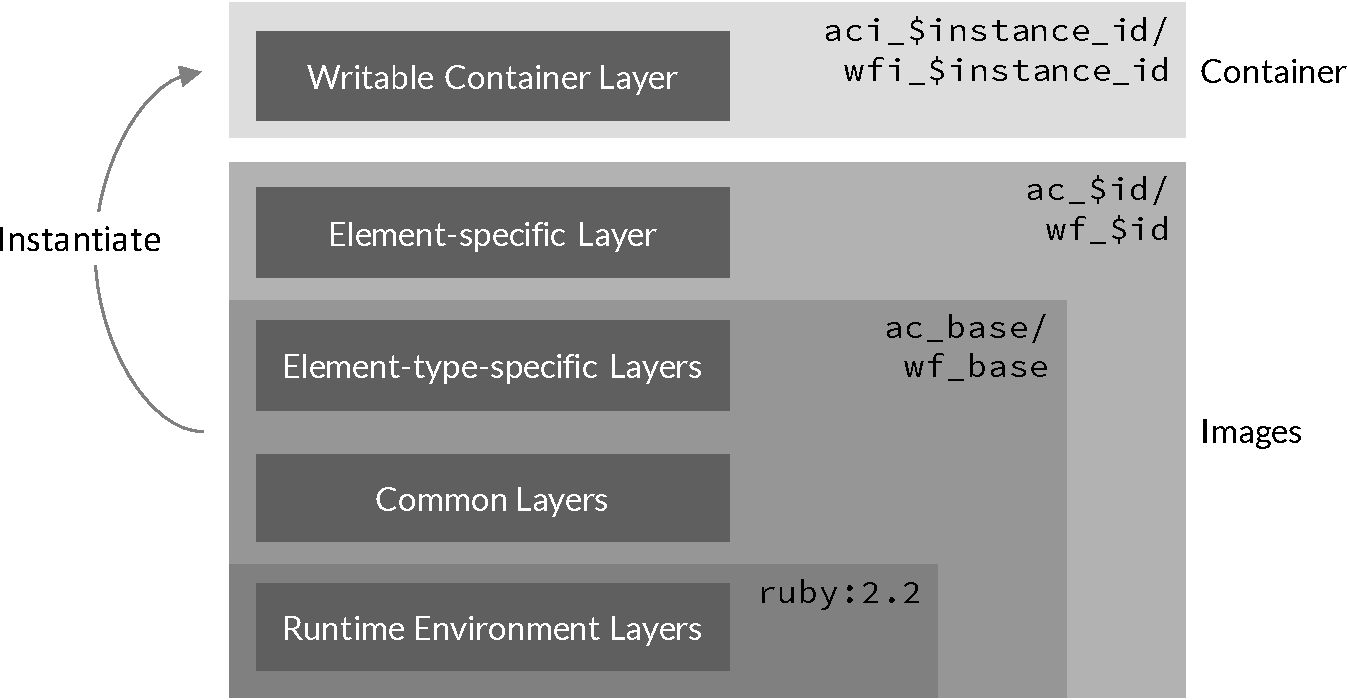
\includegraphics[width=0.95\textwidth]{content/images/layer_concept-crop.pdf}
    \caption{Layer Structure for Activity/Workflow Images}
    \label{fig:layers_for_element_wrapping_containers}
  \end{figure}

  Regarded in a more detailed fashion, the images' structure should look as follows.
  The foundation should be formed by \emph{runtime environment layers}, as they are expected to change rather seldom and are required by all derived images. Usually, these layers contain an \ac{OS}, common libraries and utility programs.

  The layers that form the \emph{$^*$\_base} images can be separated in two groups, \emph{common layers} and \emph{element-type-specific layers}. The \emph{element type} refers to either activity or workflow.
  The common layers should be created on top of these runtime environment layers. They are intended to contain the effects of invoked commands, added directory structures and files which are required by both activity images and workflow images. Even though no explicit name is given to these layers, they will be stored by Docker in its cache and used during the build process.

  In the next step, element-type-specific layers should be added. These layers are meant to contain data that is required for the execution of an activity \emph{or} a workflow, for example scripts which perform validation tasks (if they are not provided by a service) or general-purpose data transformation.

  The element-specific layer, which is added in the course of the export of an element (activity or workflow), contains files that are particular to single workflows or activities. In case of workflow images, for example, this layer would contain the process definition. In an activity image, it would contain the activity configuration and the schemata for data validation.

  By instantiating the resulting image a container is created at runtime, which owns the uppermost, writable layer. This is where the activity or workflow may store data that it needs during execution.

  At the time of writing, Docker registries do not yet reuse layers across repository borders during uploads, even though it is a proposed feature \cite{Mcgowan2015Proposal}. In order to benefit from the layering in the previously described way, it is thus necessary to let all activity images reside in the same repository by tagging them in the format

  \centerline{\texttt{\$repository\_url/activity}}

  and using the respective activity's \ac{ID} as a version tag to differentiate between them. They can then be referred to as

  \centerline{\texttt{\$repository\_url/activity:ac\_\$activity\_id}}

  Analogously, this is done with workflow images. Since it implies losing the internal image versioning mechanism, this solution should only be used as a workaround until cross-repository sharing of layers is possible.


\textcolor{red}{
  supported functions:
    - activity images
      - start subworkflow
      - start third-party container
      - initiate user input
    - workflow images
      - ggf wf engine
      - manage workdirectory (DV approaches)
}
% subsection workflow_activity_images (end)

\subsection{Communication} % (fold)
  \label{sub:application_level_communication}
  While the previous considerations were targeted at finding a model for the low-level communication, a way how the services communicate with each other

  - message queue between services
  - jeweilige protokolle via docker networks network between
  services publish/subscribe
% subsection application_level_communication (end)

  % \begin{sequencediagram}
    % \newinst{u}{Developer Gateway}
    % \newinst[1]{d}{Definition Service}
    % \newinst[1]{m}{MOM}
    % \newinst[1]{p}{Provisioner}

    % \mess{u}{subscribe}{m}
    % \mess{d}{subscribe}{m}
    % \mess{p}{subscribe}{m}

    % \mess{u}{wfms.wf.create}{m}
    % \mess{m}{wfms.wf.create}{d}
    % \mess{d}{wfms.wf.created}{m}
    % \mess{m}{wfms.wf.created}{u}
    % \mess{u}{wfms.pd.update}{m}
    % \mess{m}{wfms.pd.update}{d}
    % \mess{d}{wfms.pd.updated}{m}
    % \mess{m}{wfms.pd.updated}{u}
    % \mess{u}{wfms.wf.export}{m}
    % \mess{m}{wfms.wf.export}{d}
    % \mess{d}{wfms.wf.exported}{m}
    % \mess{m}{wfms.wf.exported}{p}
    % \mess{m}{wfms.wf.exported}{u}

  % \end{sequencediagram}

% subsection inter_component_communication (end)

\subsection{Components} % (fold)
  \label{sub:components}
  As noted in \ref{par:micro_services_architecture}, one of the downsides of \ac{MSA} is that it is crucial to determine suitable service boundaries. Some sources advise to first build a monolithic application and then analyze the result to single out services that can be extracted. In case of \acp{WfMS}, the identification of system components by the \ac{WFMC} for their reference model can be interpreted as such an analysis. Based on those components further micro-services for the prototype are then identified.

  As presented in \ref{sub:system_components}, the \ac{WFMC} identified the following components \cite[p.~13]{Hollingsworth1995Wfmc}:
    \begin{itemize}[nosep]
      \item Software Components
        \begin{itemize}[nosep]
          \item Definition Tool %
          \item Organization Modeling Tool %
          \item User Interface
          \item Workflow Engine(s)
          \item Worklists Handler %
        \end{itemize}
      \item Data Components
        \begin{itemize}[nosep]
          \item Organization Data %
          \item Process Definitions Data %
          \item Workflow Control Data
          \item Workflow Relevant Data %
          \item Worklists Data %
        \end{itemize}
    \end{itemize}

    ** draw communication diagram here **

  According to the \ac{WFMC}'s description, the definition tool, the worklists handler and the organization modeling tool each utilize a respective data component. Together with its respective datastore, each of them can be considered as an autonomous micro-service, since each would theoretically be able to provide its functionality without any further service.

  The workflow control data component can be considered as part of a workflow engine service.
  Depending on the chosen mode for the enactment, workflow relevant data is either managed by the workflow engine service, too, or accounted for by a data volume ($*_{*}^{DV}$). Only in the $*_{*}^{SER}$ variant, a dedicated service for its management and storage is needed.

  According to the decision to use the \ac{API} gateway pattern (\ref{sub:user_interaction_with_the_system}) to hide the internal system structure from its users, the two concact points -- one for administrative work and one for end-user work -- are realized using an appropriate gateway. The \emph{developer gateway} enables requests to the definition service, the infrastructure service and the organization management service through a \ac{GUI}. The \emph{user gateway} emits requests to the worklists service, wich are also issued through a \ac{GUI}.

  ** TODO: add deductions from objectives **
  In addition to the services derived above, the need for some additional services originates from considerations in \ref{sec:docker_for_wf_execution} and the objectives that were stated in \ref{sec:determination_of_objectives}.
  A Docker image registry was suggested to be used for the distribution of images to all nodes. Unless an external service such as Docker Hub is is used, an own registry service should be part of the \ac{WfMS}.
  The decision made in \ref{sub:application_level_communication} to use \ac{MOM} for the communication between services creates the need for a service which acts as such a middleware.
  To meet the requirement of automatically distributed images, a provisioning service should be introduced, which performs the appropriate actions. An infrastructure management service could be used to monitor the status and properties of the available nodes in the swarm.

  Besides the major components, independent functionalities which are frequently used could be singled out to separate services.
  %To demonstrate this exemplarily, a service which deals with the validation of input and output data is extracted for this prototype.
  One micro-service that might be extracted could for example address the validation of input and output data. Given a dataset and a set of rules on how to validate this dataset, such a service would be able to perform its task autonomously. As validation is a frequently recurring action in the execution of workflows -- before and after each activity and workflow -- it could thus be beneficial to be able to scale the execution of this task independently. **out of scope!**

  In the following, the resulting set of services is presented.

  \subsubsection{Workflow Definition Service} % (fold)
    \label{subs:workflow_definition_service}

    The workflow definition service encompasses the functions envisioned by the \ac{WFMC} as \emph{process definition tools}, \ie it is concerned with the analysis, modeling, description and documentation of business processes in form of workflow models and their process definitions. It further manages the assignment of activities to roles.

    With regards to its functional scope, the workflow definition service is also the service that should handle the transformation of workflows into their distributable format, \eg a self-contained description file or Docker images. In case of the latter, the workflow definition service would require access to a Docker daemon in order to perform the export. Once a workflow is transformed, the service should publish it. The transformations of workflows is performed by the \texttt{ImageBuilder} class, which relies on the \texttt{ProcessDefinitionImageSerializer} for the serialization of the process definition. The logic required for publishing the images is defined in the \texttt{ImageManager} class.

    The service should have \texttt{Workflow}, \texttt{Activity}, \texttt{ProcessDefinition}, and \texttt{ControlFlow} model classes, which provide the object-relational mapping for the respective objects. The roles assigned to activities have only to be dealt with in the form of unique identifiers, relying on the assumption that components which have to use them may resolve these identiefiers themselves.

    As a user interface is provided by the developer gateway service, the workflow definition service does not offer its own user interface, but rather exposes its functionality via the \ac{MOM}. This allows workflow definitions to be created and altered by arbitrary other services, \eg an conversion service which translates other process definition formats or some feedback mechanism that alters workflows based on their execution performance -- or a gateway service that provides an user interface.

    \begin{figure}[htbp]
      \centering
      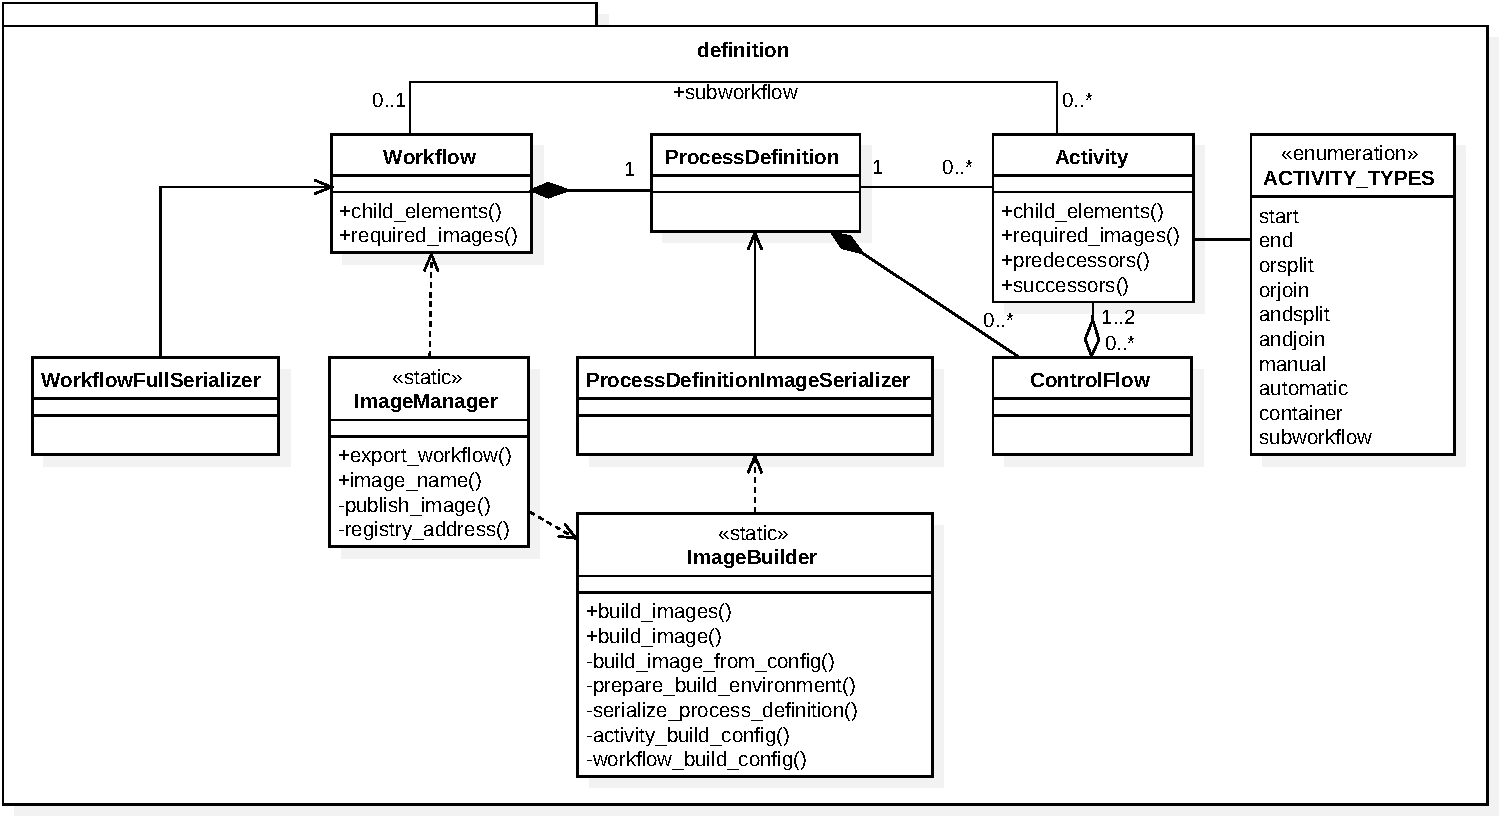
\includegraphics[width=0.95\textwidth]{content/images/class_diagram_definition-crop.pdf}
      \caption{UML Class Diagram for the Definition Service}
      \label{fig:uml_class_diagram_for_the_definition_service}
    \end{figure}

    In order react to requests of other services, the workflow definition service features consumer classes, which perform the required actions and publish a response, if required. \texttt{WorkflowConsumer}, \texttt{ActivityConsumer}, \texttt{ProcessDefinitionConsumer}, and \texttt{ControlFlowConsumer} response to \ac{CRUD} and index requests. The \texttt{WorkflowConsumer} additionally provides the means to react to requests for the export of a workflow.

    The serialization of a workflow with its components nested inside takes place in the \texttt{WorkflowFullSerializer}. Such a serialized version is required to avoid separte requests when the workflow is requested for modeling.

    Since one of the previously determined requirements for the prototype is that developers should be supported to use third-party images, the workflow definition service further reacts to relevant requests in the \texttt{DockerConsumer} by initiating a search for images with a specified name on Docker Hub.

    In order to be able to communicate with the \ac{MOM}, the workflow definition service is connected to the \texttt{wmfs\_backend} network.
    % ** As it is not actively involved in the enactment, it is not member of the \texttt{wfms\_enactment} network.
    % subsubsection workflow_definition_service (end)

  \subsubsection{Organization Management Service} % (fold)
    \label{subs:organization_management_service}
    The organization management service is part of the \emph{administration and monitoring tools}.
    As its name suggests, its functionality is aimed at the management of actors within an organization and their mutual relationships. The service may be queried for users or roles, or to authenticate users for the use of the \ac{WfMS}.

    The model classes \texttt{User} and \texttt{Role} provide the object-relational mapping for the database, while the \texttt{UserConsumer} and \texttt{RoleConsumer} classes enable the service to react to \ac{CRUD} and index requests that concern these objects.

    \begin{figure}[htbp]
      \centering
      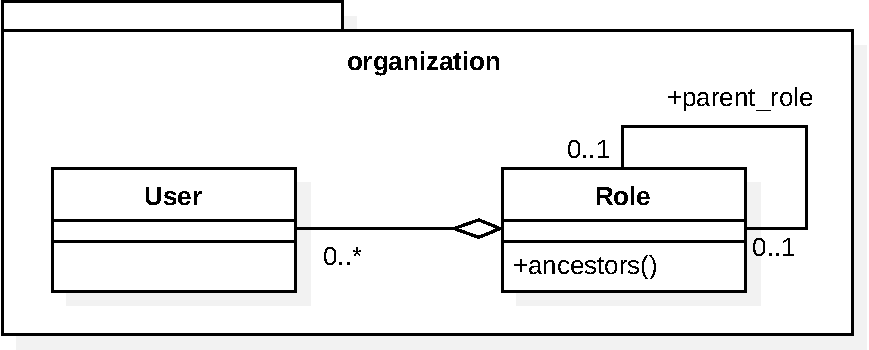
\includegraphics[width=0.65\textwidth]{content/images/class_diagram_organization-crop.pdf}
      \caption{UML Class Diagram for the Organization Service}
      \label{fig:uml_class_diagram_for_the_organization_service}
    \end{figure}

    Like the workflow definition service, the organization management service is connected to the \texttt{wmfs\_backend} network to be able to communicate with the \ac{MOM}.
    % subsubsection organization_management_service (end)

  \subsubsection{Worklist Service} % (fold)
    \label{subs:worklist_service}
    The sole responsibility of this service is the management of users' worklists. It should create, update and delete worklist items on request and publish the data submitted to it by users to the other services. If an user is deleted, it should remove the worklist item or reassign it to another user. The former tasks are performed by the \texttt{WorklistConsumer}, which reacts on related events. The latter task is in the responsibility of the \texttt{UserConsumer}, which reacts to the deletion of an user. The worklist items' object-relational mapping is performed by the \texttt{WorklistItem} model class.
    % subsubsection worklist_service (end)

  \subsubsection{Workflow Engine Service} % (fold)
    \label{subs:workflow_engine_service}
    ** TODO: incomplete **
    In wide parts, the workflow engine service is congruent to the \emph{workflow engine} component identified by the \ac{WFMC} in terms of functionality, which is described in \ref{par:workflow_engine}. The way to utilize Docker for the workflow enactment chosen in \ref{sec:docker_for_wf_execution} has an impact on the range of functionalities that this service has, though. ** like, how

    - choose participants
    - add to execution networks

    WorkflowConsumer
    WorkflowInstanceConsumer
    ServerConsumer
    WorkflowInstance
    WorkflowScheduler


    The extent to which the workflow engine service controls the instanciation of workflow components depends on .
    % subsubsection workflow_engine_service (end)

  \subsubsection{Developer Gateway} % (fold)
    \label{subs:developer_gateway}
    Since it only offers a unified access to the \ac{WfMS} and does not store any data itself, the developer gateway does not require any database. The service is realized in a two-tier architecture, with a backend part that handles requests to and responses from the various \ac{WfMS} services, and a frontend part that presents the reeived data to the developers and accepts their input.

    The only task of the backend is forwarding the user's requests to the message queue and the corresponding responses back to the user. The controller classes that are responsible for this (\texttt{ActivitesController}, \texttt{ControlFlowsController}, \texttt{DockerController}, \texttt{ProcessDefinitionsController}, \texttt{RolesController}, \texttt{ServersController}, \texttt{UsersController}, \texttt{WorkflowsController}) are thus very lean -- they only contain the logic to forward requests to suitable routing keys. Each of them inherits from the \texttt{ApplicationController}, which manages the messaging logic and gives access to a shared single connection to the \ac{MOM}.

    The \texttt{TemplatesController} is different from the other controller classes, as is not involved in forwarding requests, but serves the only purpose to render and deliver the \ac{HTML} fragments required by the frontend.

    Following the API gateway pattern, this service and the user gateway service are intended to be the only services that can be reached from outside of the \ac{WfMS}.
    ** API GATEWAY DEFINED?

    % subsubsection developer_gateway (end)

  \subsubsection{User Gateway} % (fold)
    \label{subs:user_gateway}
    Analogous to the developer gateway, the user gateway provides access to those \ac{WfMS} services that are relevant to its users, that is, in the chosen setup, only the worklist management service.

    Due to the few responsibilities of this gateway, there exist only two controller classes: \texttt{WorklistItemsController}, which forwards \ac{CRUD} requests that concern worklist items and \texttt{WorklistController}, which provides the means to obtain all existing worklists.
    % subsubsection user_gateway (end)

  \subsubsection{Infrastructure Management Service} % (fold)
    \label{subs:environment_management_service}
    The infrastructure management service fetches and refines the information related to the swarms nodes.
    That is, it lists all nodes and can return their properties, (running) containers and available images.
    Supported by the \texttt{DockerHelper}, which provides the connections to the different nodes, the \texttt{EnvironmentManager} contains the required logic to fulfil thise tasks. The \texttt{ServerConsumer} waits for relevant requests via the \ac{MOM}, instructs the \texttt{EnvironmentManager} accordingly, and returns the results. Further, there is a \texttt{Server} model class, which is used to structure the obtained information.

    Additionally to its role in the information retrieval, the \texttt{EnvironmentManager} listens for new nodes in the swarm and launches the provisioning service on joining nodes.
    % subsubsection environment_management_service (end)

  \subsubsection{Registry} % (fold)
  \label{subs:registry}
    All solutions presented in Section~\ref{sec:docker_for_wf_execution} feature custom Docker images, be it workers or contanierized activities or workflows. These images presumably contain information on business processes and other information whose disclosure should be avoided.  In order to store and distribute these images, a private registry is thus required. A possible alternative for less sensitive images could be the utilization of a private remote repository on the Docker Hub.
  % subsubsection registry (end)

  \subsubsection{Provisioning Service} % (fold)
    \label{subs:provisioning_service}
    The objectives include the reduction of administrative work. In order to prevent the user from having to distribute the Docker images required for the execution of workflows manually, a service should perform this task. This service should provision each machine with said images whenever such an image is created or updated. To do so, the \texttt{ImageConsumer} and \texttt{ServerConsumer} classes react to relevant events by invoking the appropriate Docker commands.

    The service could either run as an instance on each machine, performing the required Docker operations locally, or run on the Docker Swarm master machine as one instance and perform the operations remotely on all machines. The former variant enables all nodes to react concurrently to the event of a published image, while in the latter variant, the distribution would take place sequentially -- unless the service is implemented in a multi-threaded or multi-process way. While the idea of provisioning all nodes at the same time might be appealing, the workload imposed on the registry node by a big swarm should be considered.
    % subsubsection provisioning_service (end)
% subsection components (end)


      % section design (end)

    % section docker_in_workflow_management (end)
  % chapter solution_design (end)

  \chapter{Prototypical Implementation} % (fold)
    \label{cha:implementation}

    % -*- root: ../../main.tex -*- %

\section{Design decisions} % (fold)
\label{sec:design_decisions}
  - GDVSEPC
  - wf engine partially in wf container
  - ruby / ruby on rails for readability and because i know it
    - drawback: speed, runtime

  - extra validator
    - defeats purpose of not sending data in gdvsepc but, just POC

  - for sake of simplicity:
    - no compiled language
% section design_decisions (end)

\section{Execution Images} % (fold)
\label{sec:execution_images}

  \subsection{Workflow Image} % (fold)
  \label{sub:workflow_container}
    - application
      - process instance
      - process definition
      - activity instance
      - file helper
      - configuration

  % subsection workflow_container (end)

  \subsection{Activity Image} % (fold)
  \label{sub:activity_containers}
    - application
      - configuration
      - file helper
  % subsection activity_containers (end)

% section execution_images (end)

\section{System Components} % (fold)
\label{sec:components_implementation}
  \subsection{Workflow Definition Service} % (fold)
    \label{sub:workflow_definition_service}
      - application
        - ruby on rails (api)
        - components
          - app logic
            - dockerhelper
            - image builder
            - image manager
          - controllers
          - models
            - activity
            - control-flow
            - process-definition
            - workflow
          - serializers
            - process definition image serializer
            - workflow full serializer

      - database
        - postgresql
      - data volume
        - docker volume

    \begin{figure}[htbp]
      \centering

      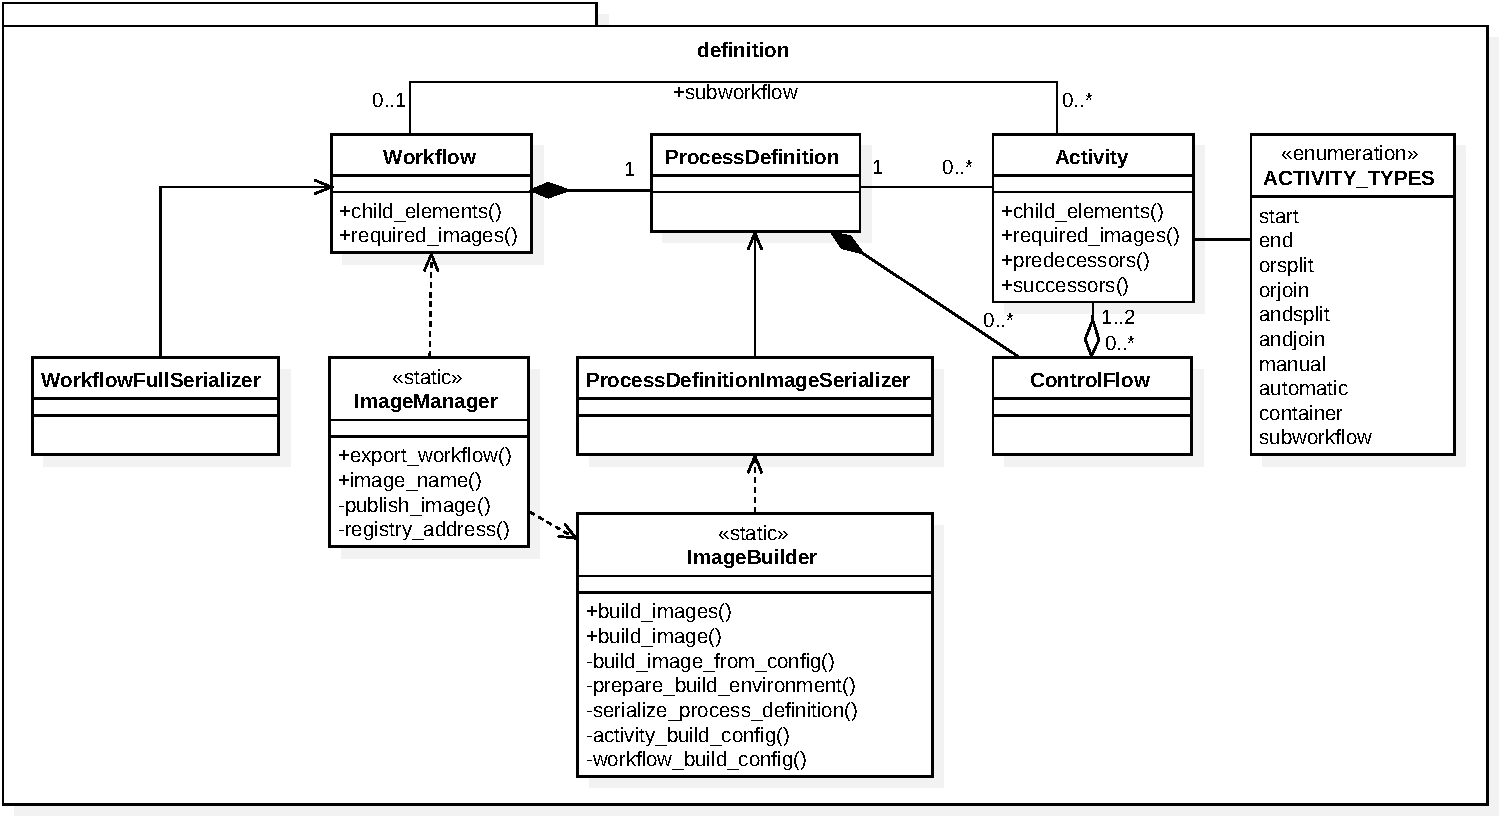
\includegraphics[width=0.95\textwidth]{content/images/class_diagram_definition-crop.pdf}
      \caption*{\scriptsize Controllers omitted for the sake of simplicity. Workflow, ProcessDefinition, Activity and ControlFlow each have a controller with the respective pluralized name plus a `Controller' suffix.}
      \caption{UML Class Diagram for the Definition Service}
      \label{fig:label}
    \end{figure}
    % subsection workflow_definition_service (end)

  \subsection{Organization Management Service} % (fold)
    \label{sub:organization_management_service}
      - application
        - controllers
        - models
          - role
            - ancestors
          - user
            - with role
      - database
        - postgresql
      - data volume
        - docker volume
    % subsection organization_management_service (end)

  \subsection{Worklist Service} % (fold)
    \label{sub:worklist_service}
      - application
        - controllers
        - models
          - worklist item
      - database
        - postgresql
      - data volume
        - docker volume
    % subsection worklist_service (end)

  \subsection{Workflow Engine Service} % (fold)
    \label{sub:workflow_engine_service}
      - application
    % subsection workflow_engine_service (end)

  \subsection{Developer Gateway} % (fold)
    \label{sub:developer_gateway}
      - application
        - backend: rails
        - frontend: angular app
    % subsection developer_gateway (end)

  \subsection{User Gateway} % (fold)
    \label{sub:user_gateway}
      - application
        - backend: rails
        - frontend: angular app
    % subsection user_gateway (end)

  \subsection{Message Oriented Middleware} % (fold)
    \label{sub:message_oriented_middleware}
      For this prototype, RabbitMQ was chosen as message oriented middleware, because it is well documented and has various ruby clients, \eg \emph{Hutch} and \emph{Bunny}.

      RabbitMQ exists as a pre-configured Docker image on the Docker Hub and can thus be utilized easily. The configuration of RabbitMQ in this image takes place when the respective container is run, which allows its configuration in the \texttt{docker-compose} configuration file.
      For the sake of simplicity, no authentication mechanism was introduced besides the simple default username/password combination.
    % subsection message_oriented_middleware (end)

  \subsection{Infrastructure Management Service} % (fold)
    \label{sub:infrastructure_management_service}
      - application
        - app logic
          - docker helper
          - environment manager
        - controllers
          - servers controller
        - models
          - server

    % subsection infrastructure_management_service (end)

  \subsection{Registry} % (fold)
    \label{sub:registry}
    % subsection registry (end)

  \subsection{Provisioning Service} % (fold)
    \label{sub:provisioning_service}
      - application
    % subsection provisioning_service (end)
% section components (end)


\begin{figure}[htbp]
  \centering
  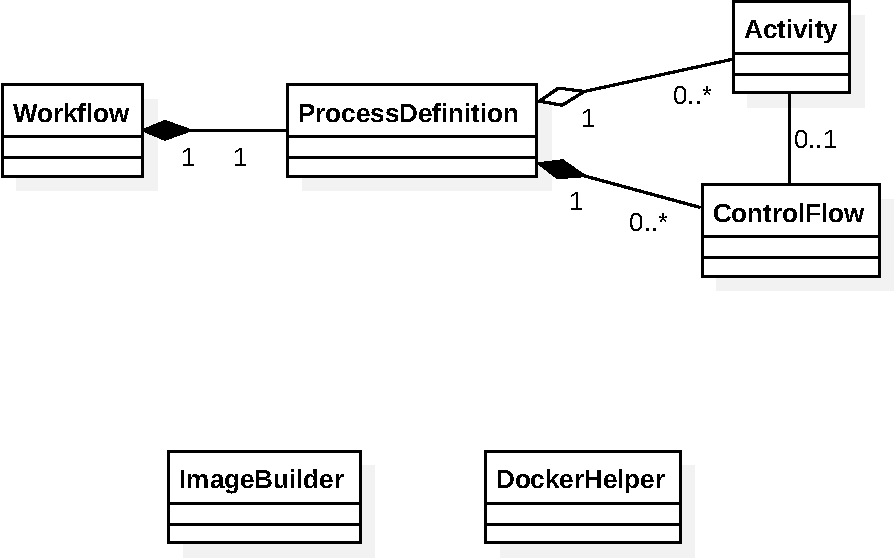
\includegraphics[width=0.95\textwidth]{content/images/class_d_definition-crop.pdf}
  \caption{UML Class Diagram for Workflowe Definition Service}
  \label{fig:uml_class_diagram_definition_service}
\end{figure}

    % chapter implementation (end)

  \chapter{Evaluation and Discussion} % (fold)
    \label{cha:evaluation}
    % -*- root: ../../main.tex -*- %

  - decision tree for wf containerization type -
  - capability table -
  - UML diagrams (classes/deployment) -
  - actual code \& Compose configuration


  In Chapter~\ref{cha:implementation}, the prototypical implementation of a Docker-based \ac{WfMS} is presented. This implementation is based on the considerations that are made in Chapter~\ref{cha:solution_design}. In that chapter, objectives for the prototypical implementation were gathered, together with the requirements that must be met in order for these objectives to be considered fulfilled.

  % Using the prototype, a developer is able to model an organization hierarchy, create workflows and define their processes graphically. These workflows can be exported to Docker containers and are then distributed to all nodes. The developer can start workflows, and -- if a manual activity is present -- a user can enter data. The developer can pause and unpause the workflow.

  In \ref{sub:application_level_communication} is explained how the loose coupling of micro-services via \ac{MOM} and the encapsulation of these services in separate containers can enable alterations to components of the \ac{WfMS} at runtime.

  Regarding the requirements that concern the failure resilience of a service, the prototype is able to let all parts of the system that do not rely on failed services continue to offer their functionality. If, for example, the organization service failed, it would still be possible to model and execute a workflow. Also, the possibility to instruct Docker to restart failed containers can help to keep the system available. In case of a micro-service failure, the unanswered requests to it remain in the queue and can be processed as soon as the service is available again. The prototype's ability to cope with failure can thus mainly be attributed to the combination of Docker with a \ac{MSA}.

  The management of nodes that are available for execution is mostly handled by Docker Swarm. By starting appropriately configured swarm agent containers on them, new nodes may be added to the swarm at any time. The infrastructure service notices the addition of new nodes and starts a provisioning service on them. This service in turn reacts to pushed images and instructs its respective node to pull them.

  The prototype supports the user in using third-party images by providing the means to search for images on the public Docker Hub registry. Further, the invoked command can be specified for utilized third-party images. The graphical modeling environment abstracts from the fact that the container is started by an intermediate activity container.

  % \textbullet ~ User can specify validation  schemas
  % \textbullet ~ \ac{WfMS} performs validity checks

  Some of the objectives were addressed in theory only, but were not implemented in the prototype.
  As described in \ref{sub:execution_scheduling}, nodes can be labeled and these labels can be used to enforce required properties of nodes for certain workflows or activities. ** for single entities?**
  The prototype applies this principle, but in a static way -- not on a dynamic, per-element level.

  Likewise, a solution for the priorization of activities and workflows was presented in \ref{} ** show it**, but it was not implemented in the prototype.

  % An objective that was disregarded in the implementation to keep the *what? thesis short?* is the management of permanently running services which are provided for specific workflows or activities. While it is theoretically described in \ref{}, there is no corresponding functionality in the prototype.

  ** GDVSEPC does not support the exchange of data between workflow instances

  **
  - considering similar functionality /w subworkflow instantiation /validation / etc.    - probably different concept of workflows better as suggested by \cite[119]{Schulze1998Services}
   - recursive structure
   - only one base image

\underline{Note by the author:} With hindsight, the chosen scope would appear too wide for a master thesis with a 70-pages-limitation, leading to shortcuts at places where more in-depth research documentation would have been warranted. Still, the eventual outcome of the paper, i.e. the ultimate decisions on software architecture and -design are founded on solid examination of the available alternatives.

    % chapter evaluation (end)

  \chapter{Conclusion} % (fold)
    \label{cha:conclusion}
    % -*- root: ../../main.tex -*- %

In the thesis at hand, mechanisms and implementation issues that arise from the utilization of Docker and its related tools in the context of \acp{WfMS} were proposed and discussed. Two general application areas for Docker were identified: Docker may influence the architecture and design of \acp{WfMS} as well as provide new ways to distribute and execute workflows.

After introducing the concepts of \ac{WfMS}, Docker and prevalent architecture styles, possibilities for the utilization of Docker for the enactment of workflows were explored. One of them which features the encapsulation of all workflow elements in separate images and a shared data volume, was chosen to be implemented. The attention was then centered on how Docker can be used to create a flexible, failure resilient \ac{WfMS}.

The outcome of these considerations was manifested in the design and implementation of a prototype in which the feasibility of a selection of these mechanisms was demonstrated. In the course of both design and implementation of the prototype, artifacts were created that can be used by succeeding researchers or \ac{WfMS} developers.

results:
  - three promising combinations for execution
  - capability table
  - WfMC model translated to docker-enabled microservices
  - statically compiled activity/workflow would be faster

outlook:
  - pause + move containers: http://blog.circleci.com/checkpoint-and-restore-docker-container-with-criu/
  - evaluate supported patterns?  http://www.workflowpatterns.com/documentation/documents/BPM-06-22.pdf
  - implement resource management


    % chapter conclusion (end)

  \bibliographystyle{plain}
  \bibliography{Remote}

  \appendix
  \AnhChapter{Kapitel}

  % \inputminted[fontsize=\footnotesize,linenos=true,numberblanklines=true,showspaces=false,breaklines=true,baselinestretch=1]{ruby}{../code/ac_base/run.rb}

  \begin{figure}[htbp]
    \inputminted[fontsize=\footnotesize,linenos=true,numberblanklines=true,showspaces=false,breaklines=true,baselinestretch=1]{json}{./content/snippets/process_definition.json}
    \caption{Exported process definition in JSON format}
    \label{fig:exported_process_definition_in_json_format}
  \end{figure}

  \begin{figure}[htbp]
    \inputminted[fontsize=\footnotesize,linenos=true,numberblanklines=true,showspaces=false,breaklines=true,baselinestretch=1]{Dockerfile}{../code/ac_base/Dockerfile}
    \caption{Dockerfile for activity base image}
    \label{fig:dockerfile_for_activity_base_image}
  \end{figure}

  \begin{figure}[htbp]
    \inputminted[fontsize=\footnotesize,linenos=true,numberblanklines=true,showspaces=false,breaklines=true,baselinestretch=1]{Dockerfile}{../code/wf_base/Dockerfile}
    \caption{Dockerfile for workflow base image}
    \label{fig:dockerfile_for_workflow_base_image}
  \end{figure}

  \begin{figure}[!htbp]
    \inputminted[lastline=50,fontsize=\footnotesize,linenos=true,numberblanklines=true,showspaces=false,breaklines=true,baselinestretch=1]{yaml}{../code/wfms.yml}
    \caption{The whole Docker Compose file of the \ac{WfMS} (1)}
    \label{fig:the_whole_docker_compose_file}
  \end{figure}

  \begin{figure}[!htbp]
    \inputminted[firstline=51,lastline=98,fontsize=\footnotesize,linenos=true,numberblanklines=true,showspaces=false,breaklines=true,baselinestretch=1]{yaml}{../code/wfms.yml}
    \caption{The whole Docker Compose file of the \ac{WfMS} (2)}
    \label{fig:the_whole_docker_compose_file}
  \end{figure}

  \begin{figure}[!htbp]
    \inputminted[firstline=99,lastline=145,fontsize=\footnotesize,linenos=true,numberblanklines=true,showspaces=false,breaklines=true,baselinestretch=1]{yaml}{../code/wfms.yml}
    \caption{The whole Docker Compose file of the \ac{WfMS} (2)}
    \label{fig:the_whole_docker_compose_file}
  \end{figure}

  \begin{figure}[!htbp]
    \inputminted[firstline=146,lastline=197,fontsize=\footnotesize,linenos=true,numberblanklines=true,showspaces=false,breaklines=true,baselinestretch=1]{yaml}{../code/wfms.yml}
    \caption{The whole Docker Compose file of the \ac{WfMS} (2)}
    \label{fig:the_whole_docker_compose_file}
  \end{figure}

  \begin{figure}[!htbp]
    \inputminted[firstline=198,fontsize=\footnotesize,linenos=true,numberblanklines=true,showspaces=false,breaklines=true,baselinestretch=1]{yaml}{../code/wfms.yml}
    \caption{The whole Docker Compose file of the \ac{WfMS} (2)}
    \label{fig:the_whole_docker_compose_file}
  \end{figure}

  \AnhSection{Unterkapitel}

\end{document}
